\chapter{Implementação}
\label{chap5}

O desenvolvimento do projeto teve início no segundo semestre de 2024, no âmbito da disciplina Software Livre e Metodologias Participativas. Após o término da disciplina, o projeto passou a integrar as atividades do projeto de extensão Tecnologia da Informação, Democracia e Movimentos Sociais (TICDeMoS), vinculado ao SOLTEC/UFRJ. Desde o início, a proposta contou com o acompanhamento da antiga gestora do PAA no PDS Osvaldo de Oliveira, que contribuiu com sua experiência para a modelagem do sistema e para a definição dos principais casos de uso.

Ao longo do desenvolvimento, a proposta passou por mudanças em sua organização técnica e funcional. Inicialmente, o sistema estava voltado para um único assentamento e com criação de uma base mínima que permitisse cadastrar usuários, famílias, produtos, ciclos, destinos e editais. Em 2025, a proposta foi apresentada à equipe da Companhia Nacional de Abastecimento do Rio de Janeiro (CONAB-RJ). Após a reunião, vimos que além do cadastro das informações essenciais do edital deveríamos contemplar o cadastro de coletivos, um painel de acompanhamento que mostrasse de forma clara o andamento do projeto e a geração de relatórios que apoiam a comprovação das entregas, visualizando valores a receber pelas famílias agricultoras, além de, facilitar a consolidação dos dados de entregas pelo coordenador.


\section{Requisitos do Sistema}

O levantamento dos requisitos do sistema foi realizado a partir de duas frentes diferentes, a primeira através de diálogo com a gestora do PAA no assentamento para entender seu dia-a-dia e como funcionava o diálogo com os agricultores e a segunda da análise baseado em planilhas no excel que mostrava o funcionamento da gestão do programa no Assentamento PDS Osvaldo de Oliveira. Inicialmente, o foco era entender como as informações das chamadas públicas eram organizadas, quais atividades eram realizadas durante a execução dos editais e quais dificuldades estavam presentes no processo de acompanhamento. Observou-se que o gerenciamento do edital envolve diferentes informações, como quais famílias agricultoras estão participando, quais produtos foram selecionados, quantas entregas foram realizadas, quais destinos receberão os alimentos e quais são os valores a receber por agricultor, além das informações para o gerenciamento do edital, era necessário gerar documentos que comprovassem as entregas.

\subsection{Casos de uso do sistema}

Os casos de uso do sistema foram definidos a partir das principais ações realizadas durante a gestão de uma chamada pública do PAA e para que ficasse coerente com o levantamento de requisitos. Como objetivo do sistema é organizar informações sobre editais, famílias, produtos, ciclos, destinos e entregas, foi necessário identificar quais pessoas interagem com a plataforma e quais atividades cada uma delas precisa realizar, que se resume em três atores principais, o administrador, o coordenador e o agricultor.

O administrador é o usuário que tem máximo acesso ao sistema, podendo criar coletivos, produtos, editais, aprovar usuários e modificar informações livremente no sistema. O segundo ator, o coordenador, é responsável por acompanhar a execução do edital, aprovar usuários do mesmo coletivo, cadastrar famílias, organizar produtos, criar editais, criar ciclos de entrega, registrar informações e acompanhar o andamento da chamada pública. Por fim, temos o agricultor que está relacionado ao acompanhamento das informações referentes à sua participação, como produtos previstos, entregas realizadas e valores a receber.

O primeiro caso de uso é o cadastro de usuários. Por meio dessa funcionalidade, uma pessoa interessada em acessar o sistema informa seus dados e solicita a criação de uma conta. Após esse cadastro, o usuário não recebe acesso imediato às funcionalidades internas, pois sua entrada depende da aprovação do coordenador/administrador.

O segundo caso de uso é a aprovação de usuários. Essa funcionalidade permite que o coordenador visualize os usuários cadastrados do mesmo coletivo e aprove ou rejeite o acesso à plataforma. Essa etapa é crucial para manter a segurança do sistema e garantir que apenas pessoas vinculadas ao processo de participação no PAA possam acessar as informações.

Outro caso de uso central é o cadastro e gerenciamento de famílias. Essa funcionalidade permite registrar as famílias agricultoras no sistema, editar suas informações e associar usuários a uma determinada família. Esse vínculo é necessário para que o sistema consiga relacionar as entregas, os produtos e os valores a cada unidade produtiva.

O sistema também possui o caso de uso relacionado à criação e gerenciamento de editais. O edital representa a chamada pública do PAA e reúne as principais informações do processo. A partir dele, são organizados os produtos, os destinos, os ciclos e as entregas.

O cadastro de produtos no sistema também é um dos principais casos de uso. Nele, o administrador registra os produtos que fazem parte do sistema e que são utilizados para a vinculação a um edital.

O cadastro de destinos também compõe os principais casos de uso. Essa funcionalidade permite registrar as organizações e equipamentos de segurança alimentar que receberão os alimentos.

A criação de ciclos de entrega é outro caso de uso fundamental. Como as entregas do PAA ocorrem de forma periódica, geralmente semanal, o sistema precisa organizar o edital em ciclos. Cada ciclo representa uma etapa de entrega e permite registrar os produtos movimentados em determinado período.

O registro das entregas realizadas representa uma das funcionalidades mais importantes do sistema. Por meio desse caso de uso, o coordenador informa quais famílias entregaram produtos, quais produtos foram entregues, em quais quantidades e para quais destinos. A partir desses dados, o sistema pode consolidar informações sobre o andamento do edital e calcular os valores correspondentes.

Também foi definido o caso de uso de acompanhamento do edital por meio de um dashboard. Esse dashboard tem como objetivo apresentar de forma visual e organizada o andamento da chamada pública, indicando informações como produtos entregues, valores acumulados, famílias participantes e ciclos já realizados.


A Tabela~\ref{tab:casos-uso-sistema} apresenta uma síntese dos casos de uso identificados para o sistema.

\begin{table}[H]
\centering
\caption{Principais casos de uso do sistema}
\label{tab:casos-uso-sistema}
\begin{tabular}{|p{4cm}|p{5cm}|p{6cm}|}
\hline
\textbf{Ator} & \textbf{Caso de uso} & \textbf{Descrição} \\ \hline

Agricultor & Solicitar cadastro & Permite que uma pessoa solicite acesso ao sistema. \\ \hline

Coordenador/\newline Administrador & Aprovar usuário & Permite aprovar ou rejeitar usuários cadastrados na plataforma. \\ \hline

Coordenador/\newline Administrador & Gerenciar famílias & Permite cadastrar, editar e organizar as famílias agricultoras participantes. \\ \hline

Coordenador/\newline Administrador  & Criar edital & Permite cadastrar uma chamada pública do PAA e suas informações principais. \\ \hline

Administrador & Gerenciar produtos & Permite cadastrar os produtos previstos no edital \\ \hline

Administrador & Gerenciar destinos & Permite cadastrar as organizações e equipamentos que receberão os alimentos. \\ \hline

Coordenador/\newline Administrador & Criar ciclos de entrega & Permite organizar o edital em períodos de entrega. \\ \hline

Coordenador/\newline Administrador & Registrar entrega & Permite registrar os produtos entregues pelas famílias em cada ciclo. \\ \hline

Coordenador/\newline Administrador & Acompanhar dashboard & Permite visualizar o andamento do edital por meio de indicadores. \\ \hline

Coordenador/\newline Administrador & Gerar relatórios & Permite gerar documentos com informações sobre entregas, produtos e valores. \\ \hline

Agricultor & Consultar informações da participação & Permite acompanhar produtos entregues, quantidades registradas e valores a receber. \\ \hline

Administrador & Manter o sistema & Permite realizar ajustes, correções e evolução da plataforma. \\ \hline

\end{tabular}
\end{table}

\section{Modelagem do domínio e estrutura dos dados}

A modelagem do domínio foi construída a fim de atender as demandas necessárias para o acompanhamento do edital. O edital foi definido como uma das entidades centrais do sistema, pois representa a chamada pública que será gerenciada. Diretamente associado ao edital nós temos o plano original, entidade que contém os produtos previstos, os destinos das entregas e as famílias participantes. 

O plano original é uma entidade que formaliza o início do edital, com informações essenciais como quais famílias irão participar, quais produtos e quais serão os destinos dos alimentos.

As famílias representam um grupo de usuários agricultores que participam do PAA. Dentro dos usuários pertencentes a família temos a entidade representante para sinalizar qual dos usuários será o responsável pelos registros nos relatórios gerados. Essa relação é importante porque as entregas e os valores a receber precisam ser vinculados corretamente ao responsável da família pela produção. 

A entidade produto representa cada alimento que faz parte da chamada pública. No sistema, os produtos podem ser cadastrados independentemente como valores globais no sistema e podem ser associados ao edital com informações como valor unitário e quantidade prevista. Essa associação permite diferenciar os produtos dos diversos editais, controlar o que foi planejado e comparar posteriormente com o que foi efetivamente entregue.

Os destinos representam as organizações, instituições ou equipamentos de segurança alimentar que recebem os alimentos. O registro dos destinos permite acompanhar para onde os produtos estão sendo encaminhados e quanto cada destino irá receber.

Os ciclos de entrega foram modelados para representar a periodicidade das entregas realizadas durante a execução do edital. Como as chamadas públicas podem envolver entregas semanais ao longo de vários meses, a divisão em ciclos permite organizar melhor o acompanhamento do processo. Cada ciclo corresponde a um período específico e pode reunir diferentes entregas, produtos, famílias e destinos.

A entrega representa o registro efetivo dos produtos fornecidos em determinado ciclo. Por meio dela, o sistema armazena quais produtos foram entregues, em quais quantidades, por quais famílias e para quais destinos. Essa entidade é uma das mais importantes para o funcionamento do sistema, pois permite acompanhar a execução real do edital e gerar informações consolidadas para relatórios e conferência dos valores a receber.

Durante a modelagem, também foi identificada a necessidade de incluir o conceito de coletivo. Essa entidade permite representar agrupamentos internos de famílias ou agricultores, respeitando a forma de organização da comunidade. Com isso, o sistema não fica limitado a uma estrutura individualizada, podendo representar formas coletivas de participação e organização da produção.

Assim como a entidade de famílias, após o levantamento de requisitos, nasceu a necessidade de inserir representantes nas entidades de destino e coletivos, pois além de serem necessárias as informações dos representantes em relatórios, o sistema registra uma relação formal de quem coordena o edital.

A Figura~\ref{fig:modelo-dominio} apresenta uma proposta de modelo de domínio simplificado do sistema, destacando as principais entidades e suas relações.

\begin{figure}[H]
    \centering
    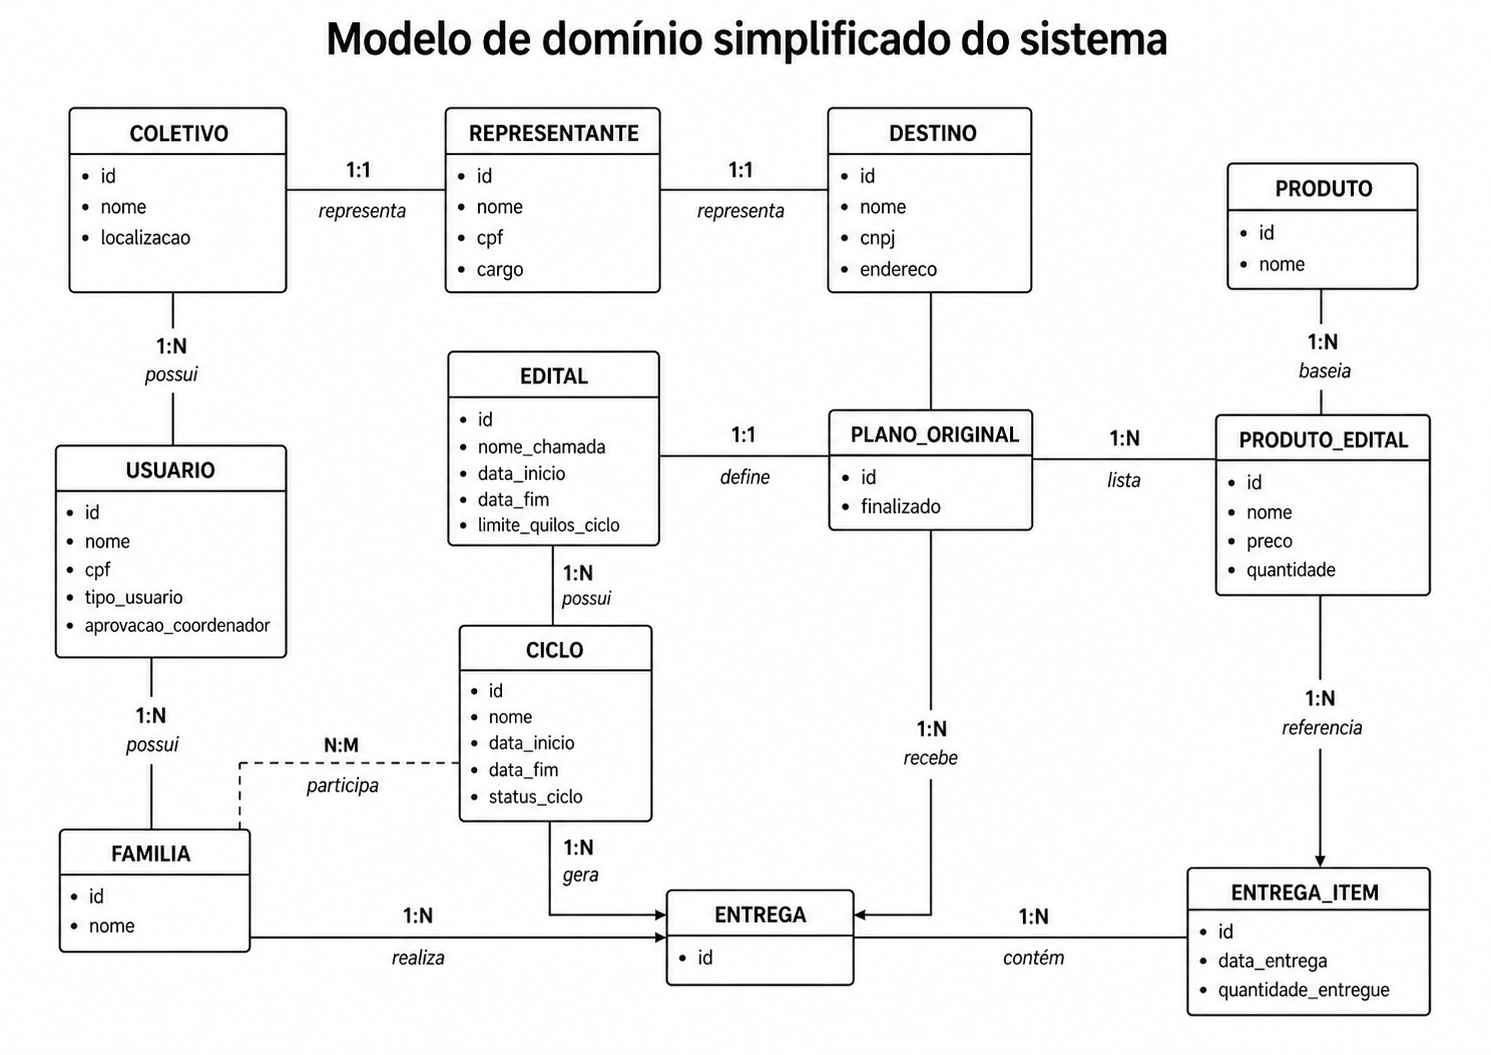
\includegraphics[width=1\textwidth]{Imagens/chap05/modelagem-diagrama-relacionamento.png}
    \caption{Modelo de domínio simplificado do sistema}
    \label{fig:modelo-dominio}
\end{figure}


\section{Arquitetura geral do sistema}

A arquitetura geral do sistema foi pensada para organizar o desenvolvimento em partes bem definidas, separando a interface utilizada pelos usuários das regras de negócio e do armazenamento das informações. Como o sistema precisa lidar com módulos e cada um com sua respectiva função, a aplicação foi estruturada para permitir que cada parte evolua de forma mais organizada, sem que uma alteração em uma funcionalidade comprometa todo o sistema.

O sistema foi desenvolvido como uma aplicação web, pois esse formato facilita o acesso por diferentes dispositivos, como computadores, notebooks e celulares.

Um ponto considerado na arquitetura foi a necessidade de manter o sistema preparado para novas funcionalidades, a arquitetura foi pensada de forma modular, permitindo que novos módulos sejam incorporados progressivamente, sem afetar o comportamento atual do sistema.

A estrutura geral é composta por duas partes principais: o frontend e o backend. O frontend é responsável pela interface com o usuário, apresentando as telas, formulários, tabelas e informações necessárias para a gestão do PAA. O backend é responsável por receber as requisições da interface, aplicar as regras de negócio e realizar a comunicação com o banco de dados. 

A intenção de manter o frontend e o backend separados era de dar independência ao desenvolvimento de cada um. Mesmo que um complete o outro, funcionalidades como filtros podem ser aplicadas ao backend sem que seja necessário derrubar toda a aplicação.

\section{Implementação do backend}

Seguindo princípios de arquitetura limpa, a estrutura de pastas do backend foi dividida em application, domain, infrastructure e web. A application é responsável pelas interfaces dos services que serão implementados. O domain representa todas as entidades do sistema que foram explicadas em seções anteriores, assim como DTOs e as interfaces que são implementadas em tempo de execução para o armazenamento no banco de dados. A infrastructure é responsável por armazenar configurações necessárias, a implementação dos services que dão a alma para o sistema e funções utilitárias para o sistema. A pasta web é responsável por armazenar os controllers que são o ponto de entrada das requisições, sejam elas vindas do frontend ou de alguma ferramenta que realiza requisições HTTP. Na Figura~\ref{fig:directory-structure} temos a ilustração da organização de diretórios do projeto.

\begin{figure}[H]
    \centering
    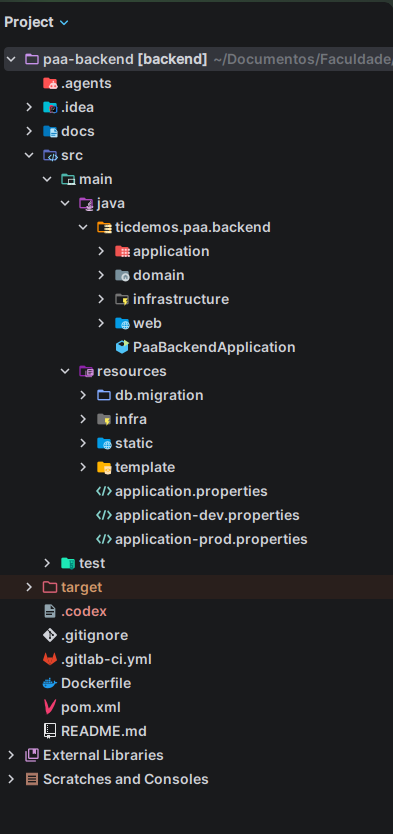
\includegraphics[width=0.5\textwidth]{Imagens/chap05/structure-directory.png}
    \caption{Estrutura de diretórios do backend}
    \label{fig:directory-structure}
\end{figure}

A tecnologia utilizada para implementar o backend foi o Java 17, juntamente com o framework Spring Boot 3. Essa escolha permitiu estruturar a aplicação de forma modular, facilitando a criação de APIs, a organização das regras de negócio e a integração com o banco de dados. Para a criação dos endpoints e dos controllers responsáveis por receber as requisições da interface, foi utilizado o Spring Web, que permitiu organizar as rotas HTTP utilizadas pelo frontend.

Para melhorar a experiência de desenvolvimento e simplificar a comunicação com o banco de dados, foi utilizado o Spring Data JPA em conjunto com o Hibernate, uma ferramenta de mapeamento objeto-relacional (ORM). Com o uso dessas tecnologias, as entidades do sistema podem ser representadas por classes Java, permitindo que operações de armazenamento e consulta sejam realizadas por meio de métodos e repositórios da aplicação. Dessa forma, reduz-se a necessidade de escrever comandos SQL diretamente.

O banco de dados escolhido foi o PostgreSQL, por ser uma ferramenta open-source, robusta e amplamente utilizada em aplicações web. Além disso, o PostgreSQL oferece bom desempenho tanto para sistemas em estágio inicial, como MVPs, quanto para aplicações maiores, que exigem maior consistência, confiabilidade e capacidade de expansão. Durante o desenvolvimento, o pgAdmin foi utilizado como ferramenta de apoio para visualizar tabelas, acompanhar registros e verificar informações armazenadas no banco de dados.

Para lidar com questões de segurança da aplicação, foi inserido no projeto o Spring Security, possibilitando o controle de acesso às rotas restritas e o bloqueio de endpoints para usuários não autenticados. Além disso, foi adotado o uso de JWT, permitindo que as requisições ao backend fossem realizadas de forma autenticada e associadas ao usuário logado. Com isso, tornou-se possível controlar o acesso às funcionalidades do sistema de acordo com o perfil de cada usuário.

Para os testes unitários, foram utilizadas as bibliotecas JUnit e Mockito. O JUnit permite estruturar e executar os testes automatizados, enquanto o Mockito possibilita simular comportamentos de componentes da aplicação, como serviços e repositórios. Essas ferramentas contribuem para validar processos críticos, como criação, atualização e consulta de dados, além de ajudar a garantir que mudanças futuras no código não comprometam comportamentos já implementados. O gerenciamento das dependências, a execução dos testes e a geração do pacote da aplicação foram organizados por meio do Maven, mantendo uma estrutura padronizada para o projeto backend.

Na documentação da API, foi utilizado o OpenAPI/Swagger, por ser uma ferramenta open-source que gera uma interface interativa para visualização e teste dos endpoints da aplicação. Com isso, torna-se possível consultar os recursos disponíveis, verificar os parâmetros esperados e testar requisições diretamente pela própria aplicação, sem a necessidade inicial de ferramentas externas. 

\section{Implementação do frontend}

O frontend foi pensado para tornar o sistema intuitivo e facilitar o uso pelos diferentes perfis de usuários. No caso do coordenador e do administrador, a interface busca auxiliar na administração dos editais do PAA. Já para o agricultor, o objetivo é permitir o acompanhamento claro do andamento de sua participação no edital.

No desenvolvimento das telas e dos componentes do sistema, foi utilizada a biblioteca React 19. Para personalizar a interface e aproximar o projeto dos padrões visuais presentes em aplicações web atuais, foi escolhida a biblioteca MUI. Além de ser open-source, essa biblioteca implementa os princípios do Material Design, proposto pelo Google, contribuindo para a construção de uma interface padronizada, responsiva e de fácil utilização. A estilização dos componentes também utiliza o Emotion, tecnologia associada ao ecossistema do MUI e utilizada para organizar estilos aplicados à interface.

O TypeScript está presente em todo o desenvolvimento do frontend, pois contribui para manter maior coerência entre os dados manipulados pela aplicação. Como o sistema realiza troca constante de informações com o backend, os dados recebidos e enviados são tipados, o que reduz erros durante o desenvolvimento e facilita a manutenção do código.

Além da biblioteca de design, o frontend utiliza outras ferramentas importantes para a organização da aplicação. O roteamento das páginas é realizado com o React Router DOM, permitindo controlar a navegação entre as diferentes telas do sistema. Para o gerenciamento de estado, são utilizados o Redux Toolkit e o React Redux, que centralizam o estado da aplicação em uma store e organizam as alterações por meio de actions e reducers. Essa abordagem contribui para tornar o comportamento da interface mais previsível, principalmente em telas que dependem de dados compartilhados entre diferentes componentes.

A comunicação com o backend é feita por meio da biblioteca Axios, responsável por realizar requisições HTTP para a API do sistema. Também são utilizadas bibliotecas auxiliares para formatação e processamento de datas, contribuindo para a apresentação adequada das informações ao usuário. O Vite foi utilizado como ferramenta de desenvolvimento e construção do frontend, facilitando a execução local da aplicação e a geração dos arquivos de produção. Além disso, o ESLint foi utilizado para auxiliar na padronização do código e na identificação de problemas durante o desenvolvimento. Todas as bibliotecas utilizadas no frontend são gerenciadas pelo arquivo package.json, por meio do npm, que organiza as dependências necessárias para o funcionamento e a manutenção da aplicação.

\subsection{Telas implementadas}

Abaixo serão apresentadas as telas do sistema, juntamente com as descrição de cada uma. Na figura~\ref{fig:login} temos a primeira tela, a de login, onde os usuários já cadastrados podem inserir suas credenciais e realizar o acesso e os interessados no sistema podem requisitar o acesso através do botão de criar conta.


\begin{figure}[H]
    \centering
    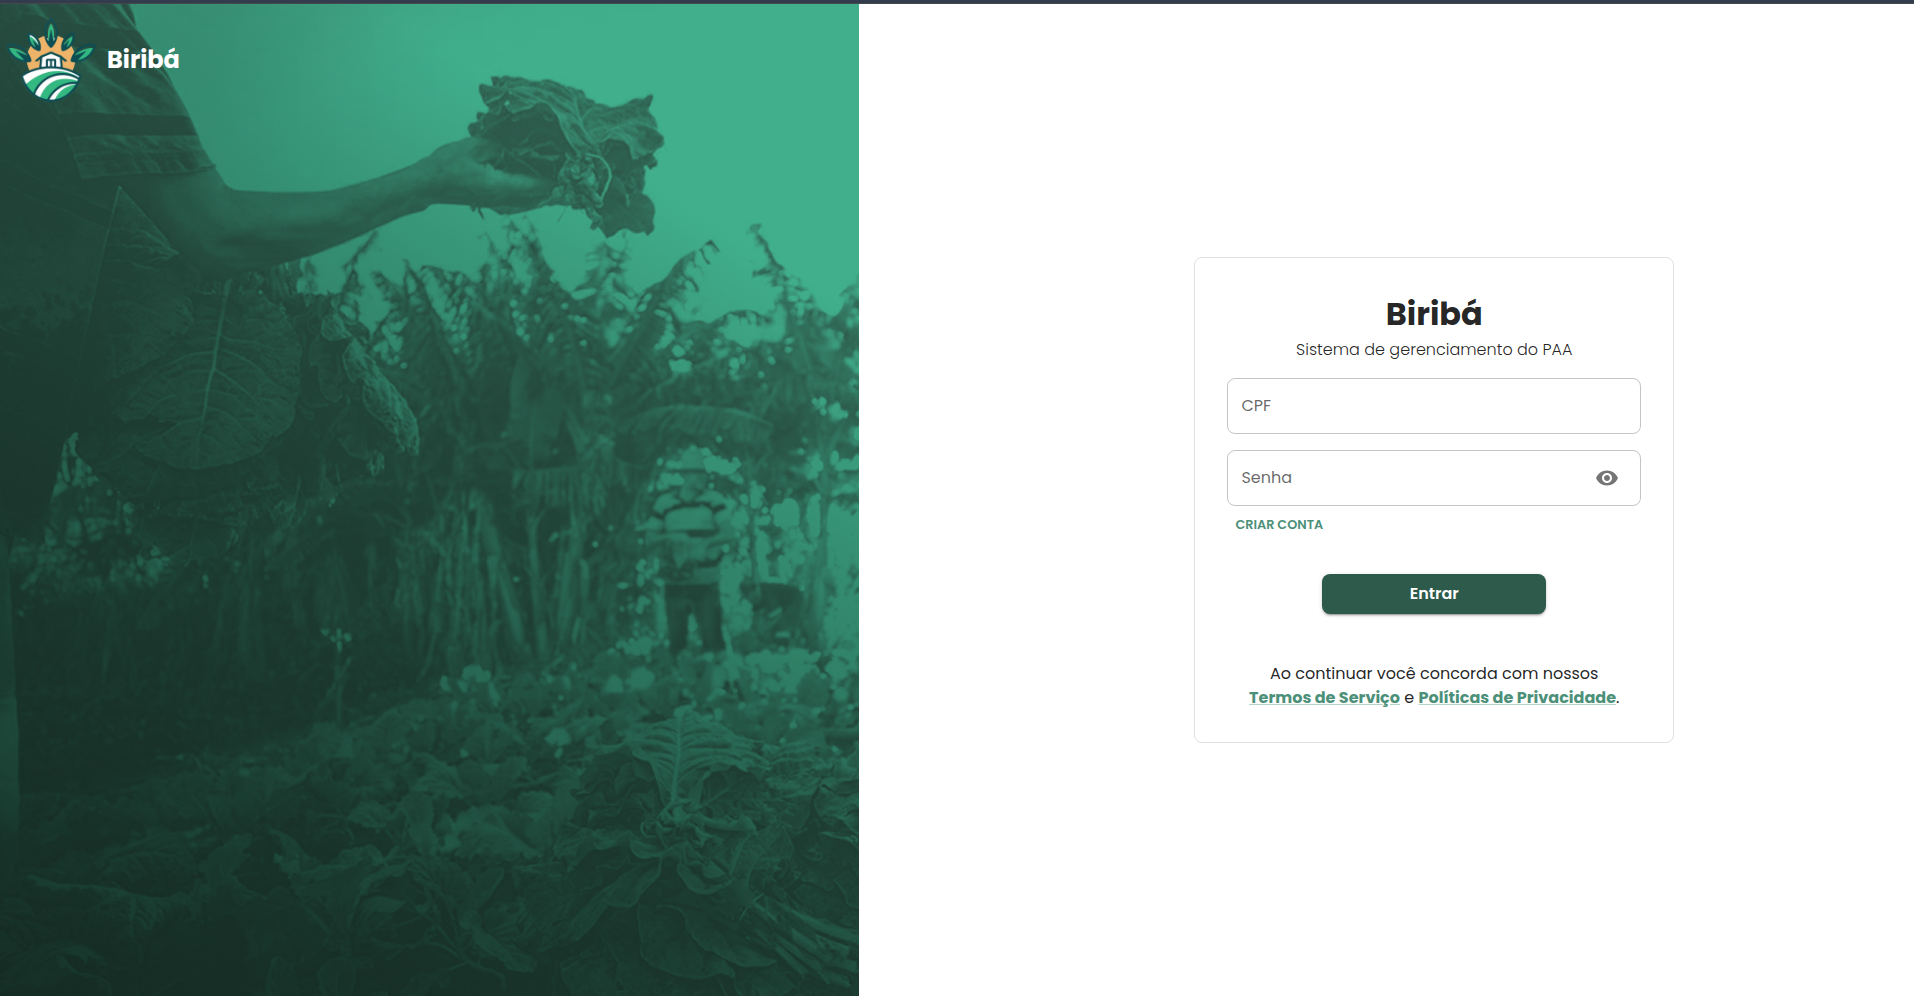
\includegraphics[width=1\textwidth]{Imagens/chap05/login_biriba.png}
    \caption{Login do sistema}
    \label{fig:login}
\end{figure}

Após o login o usuário segue para a seleção do edital que, no caso do coordenador, deseja verificar o andamento ou realizar o gerenciamento. Na tela~\ref{fig:editais} temos todos os editais disponíveis para a seleção. Vale ressaltar que o coordenador só pode acompanhar o andamento dos editais que são do seu coletivo. Um filtro é realizado no backend para que os dados que apareçam na interface sigam essa regra. O administrador do sistema pode ver todos os editais existentes, e o agricultor tem acesso semelhante ao do coordenador, podendo ver somente os editais dos quais participa. Nesta tela também podemos ver um botão de criar novos editais, permitindo que o coordenador ou o administrador inicie o gerenciamento de uma nova chamada pública.

\begin{figure}[H]
    \centering
    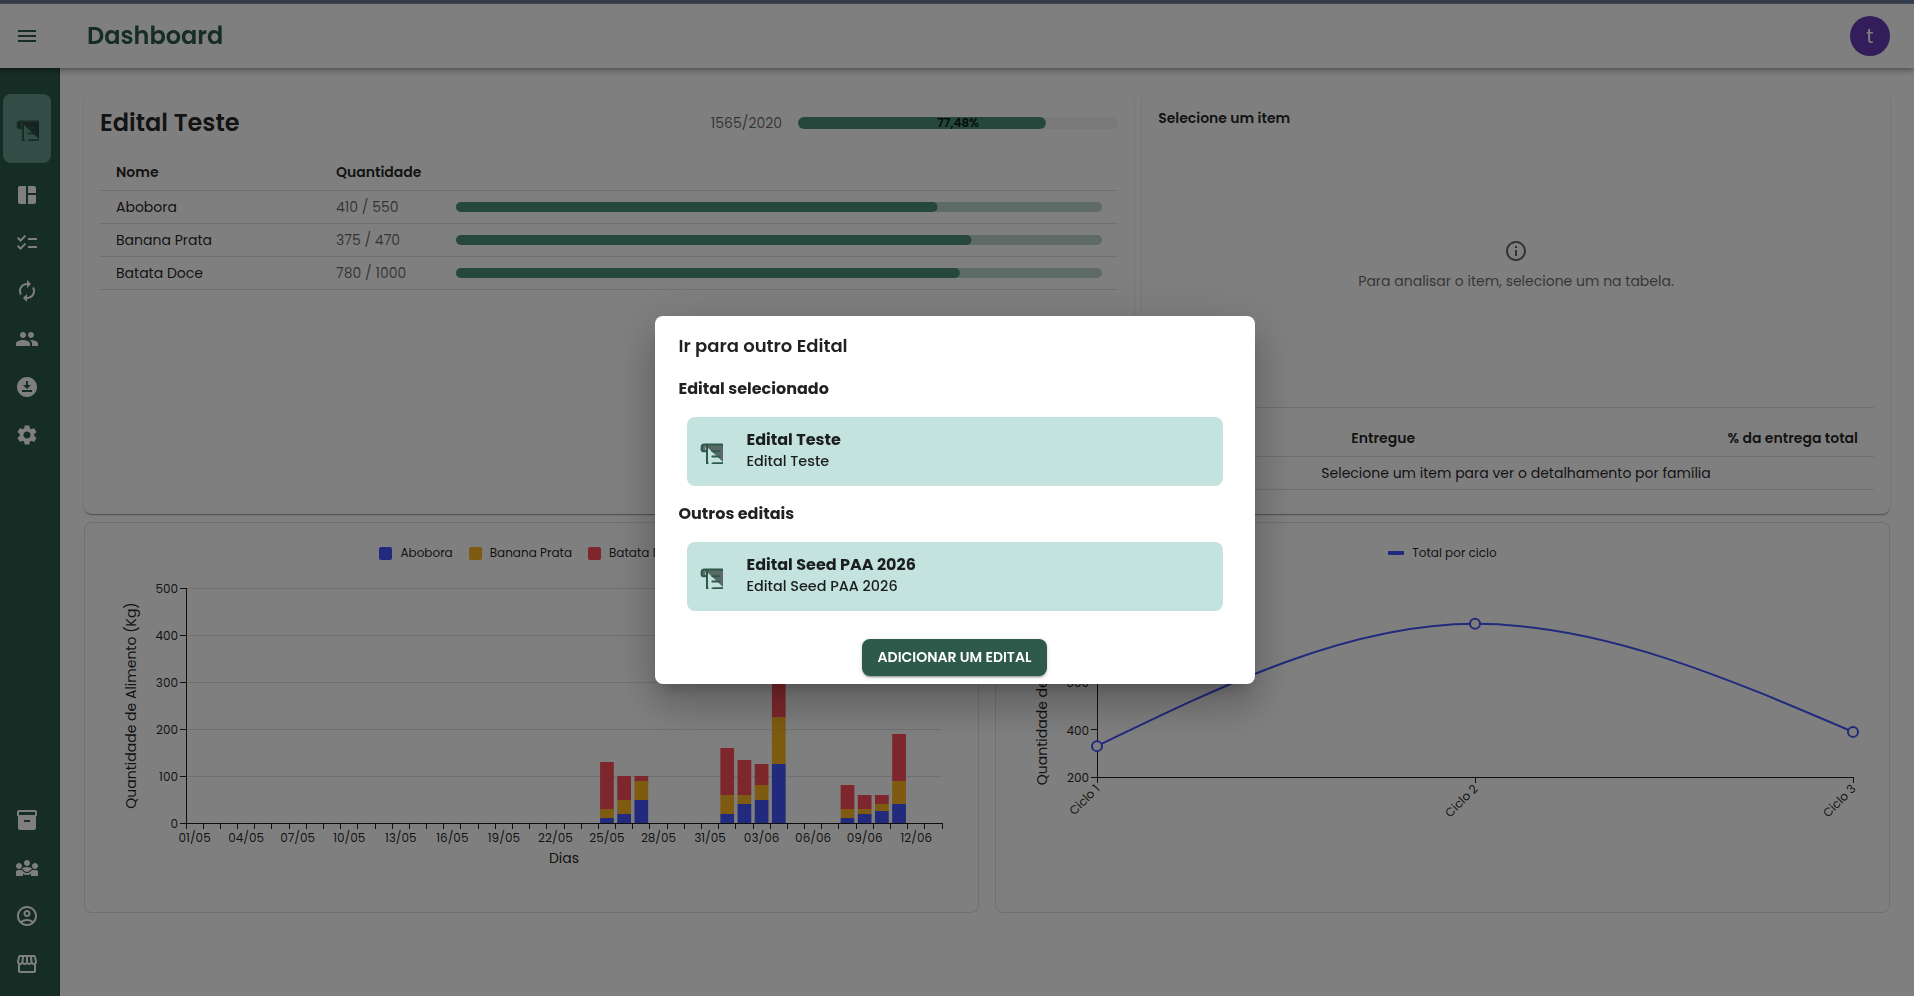
\includegraphics[width=1\textwidth]{Imagens/chap05/selecao_edital.png}
    \caption{Seleção de editais}
    \label{fig:editais}
\end{figure}

Em seguida, na criação do edital, o coordenador deverá preencher o plano original, definindo quais famílias participarão do edital, quais produtos serão ofertados e quais serão os destinos das entregas. A Figura~\ref{fig:plano-original-vazio} exemplifica um plano original parcialmente preenchido, contendo apenas as famílias e os produtos. Nessa mesma figura, observa-se a presença de botões para adicionar uma nova família ao edital e para incluir um novo produto.

Na Figura~\ref{fig:plano-original-preenchido}, é apresentada a aba de produtos por família já preenchida no plano original. A primeira coluna da tabela corresponde aos produtos que farão parte do edital selecionado, enquanto a segunda coluna indica o valor do quilo de cada produto. As demais colunas, com exceção da última, representam as famílias participantes do edital.

Em cada linha, as células associadas às famílias indicam a quantidade de determinado produto que cada família deverá entregar ao longo do edital. A última coluna apresenta o valor total, em reais, correspondente à quantidade total prevista para aquele produto. Já a última célula de cada coluna referente às famílias mostra o valor total que cada família deverá receber ao final do edital. Por fim, a célula localizada na última linha e na última coluna da tabela apresenta o valor total previsto para o edital, considerando todos os produtos e todas as famílias participantes.

Na Figura~\ref{fig:plano-original-destino}, é apresentado um exemplo de preenchimento da aba de produtos por destino. Essa tabela possui estrutura semelhante à aba anterior, mas, nesse caso, as colunas representam os destinos das entregas. Cada célula das colunas de destino indica a quantidade de determinado produto que será enviada para aquele destino ao longo do edital.

A última coluna dessa tabela é utilizada como referência para orientar o coordenador na distribuição dos produtos entre os destinos. Ela é preenchida a partir das quantidades previamente definidas para os agricultores na aba de produtos por família, permitindo verificar quanto de cada produto ainda precisa ser distribuído. Dessa forma, o coordenador consegue organizar a destinação dos alimentos de acordo com o total previsto no plano original.

Na página do plano original, além dos botões para adicionar produtos, famílias e destinos, há também o botão “Finalizar Plano Original”. Esse botão tem como objetivo encerrar a etapa de edição das tabelas e dar início ao andamento do edital. Após a finalização, as tabelas deixam de permitir alterações, garantindo que os dados definidos no plano original sejam preservados durante a execução do edital.

Observa-se que, nas Figuras~\ref{fig:plano-original-preenchido} e~\ref{fig:plano-original-destino-completo}, esse botão aparece desabilitado, e os botões de inclusão não estão presentes na tela. Isso indica que o plano original já foi finalizado e que a edição das informações foi bloqueada.


\begin{figure}[H]
    \centering
    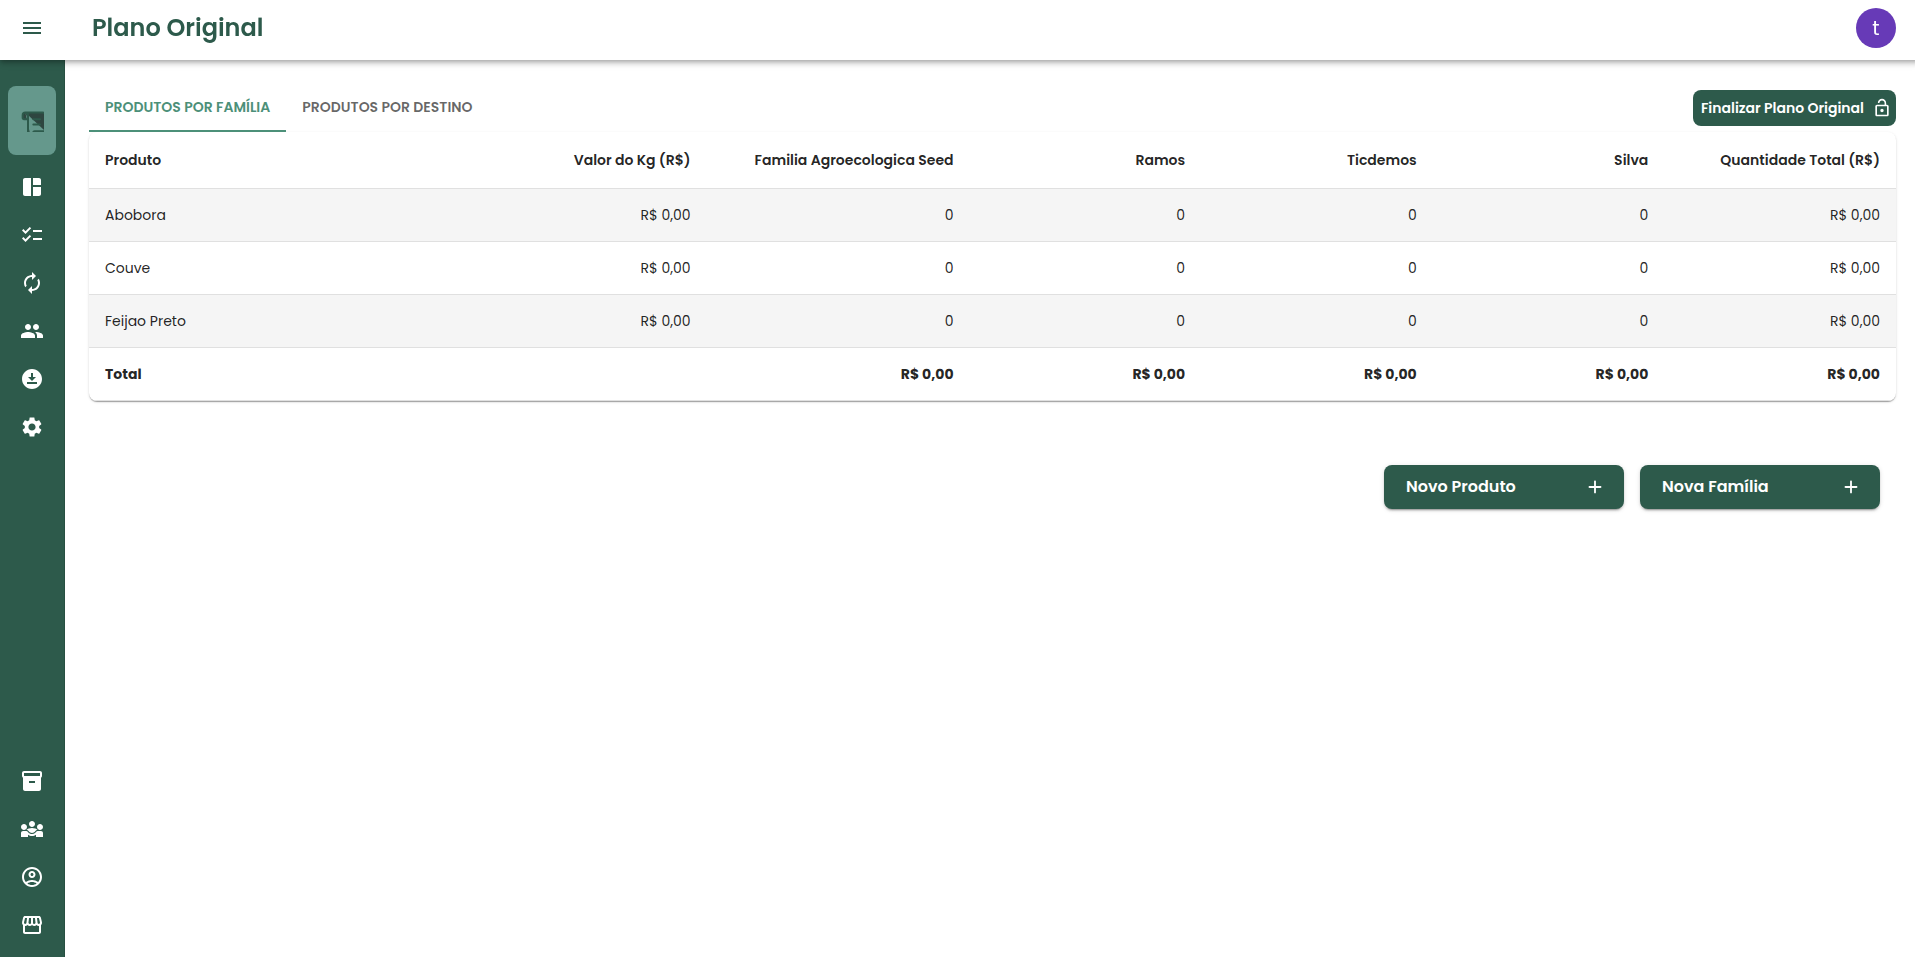
\includegraphics[width=1\textwidth]{Imagens/chap05/plano_original_vazio.png}
    \caption{Plano original aba produto por família parcialmente preenchido}
    \label{fig:plano-original-vazio}
\end{figure}

\begin{figure}[H]
    \centering
    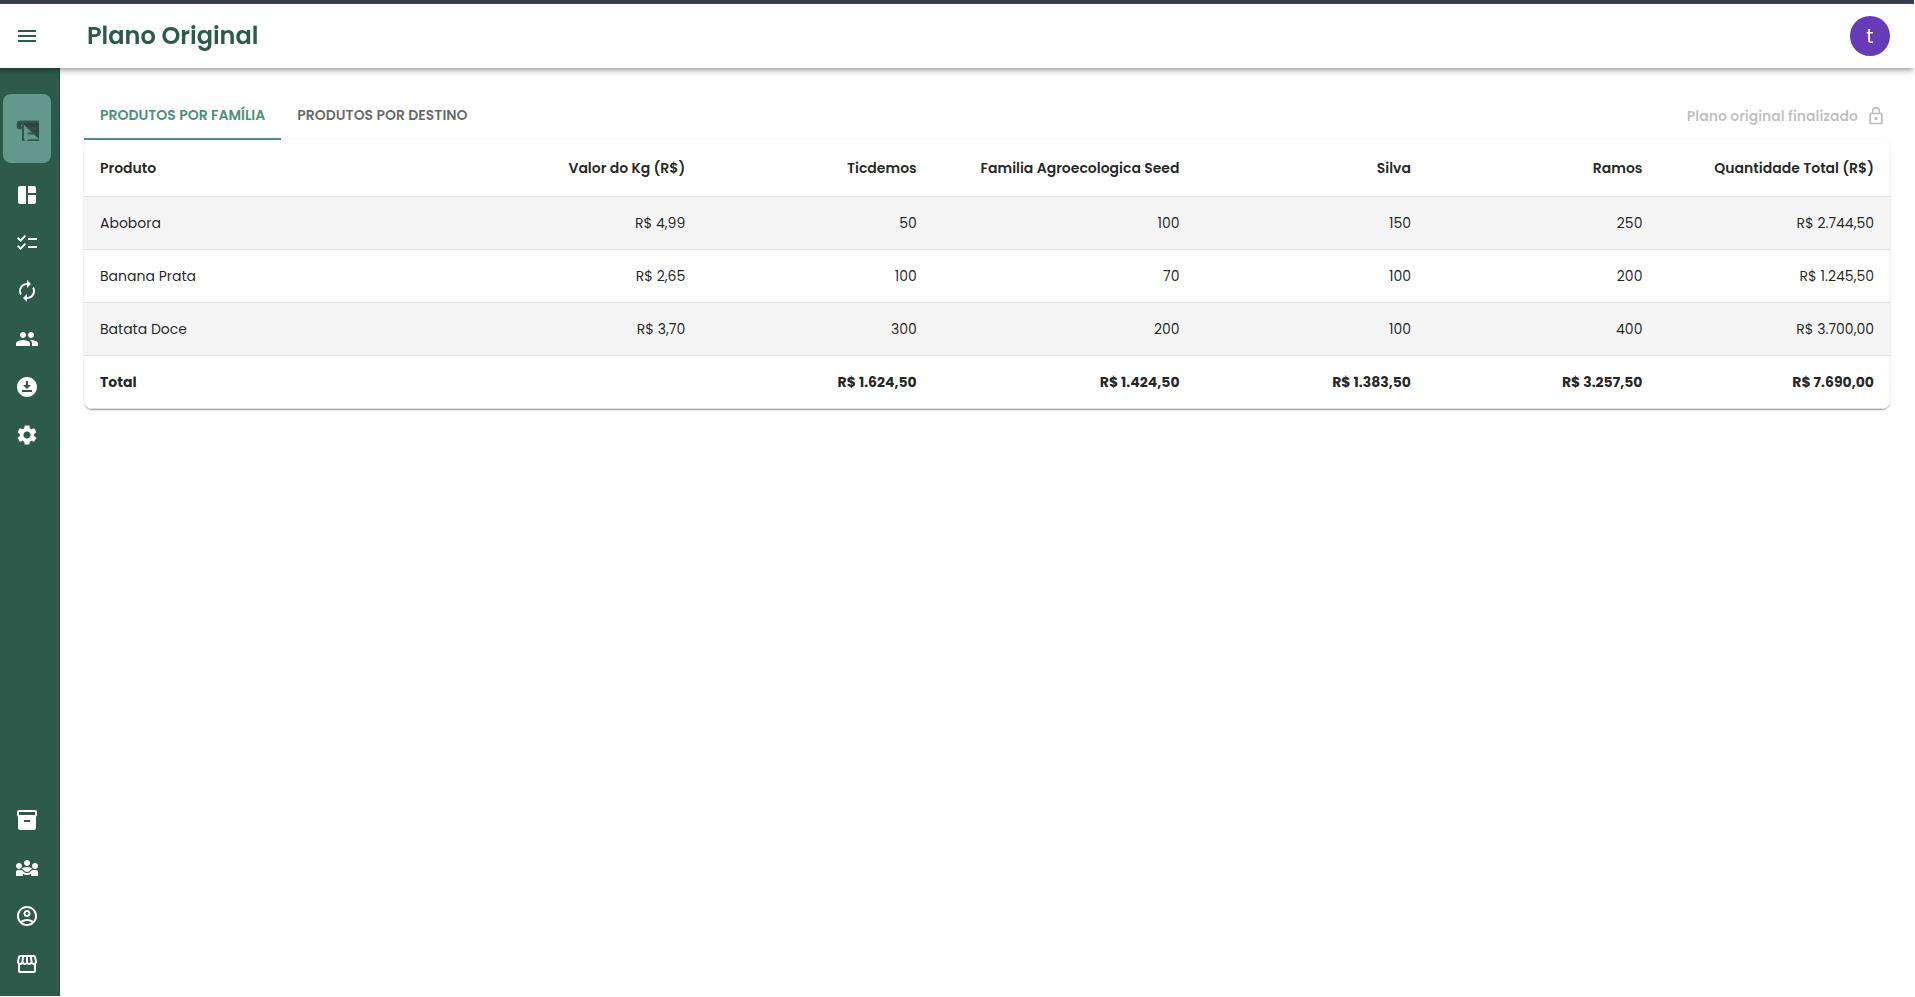
\includegraphics[width=1\textwidth]{Imagens/chap05/tela_plano_original.png}
    \caption{Plano original aba produto por família completo}
    \label{fig:plano-original-preenchido}
\end{figure}

\begin{figure}[H]
    \centering
    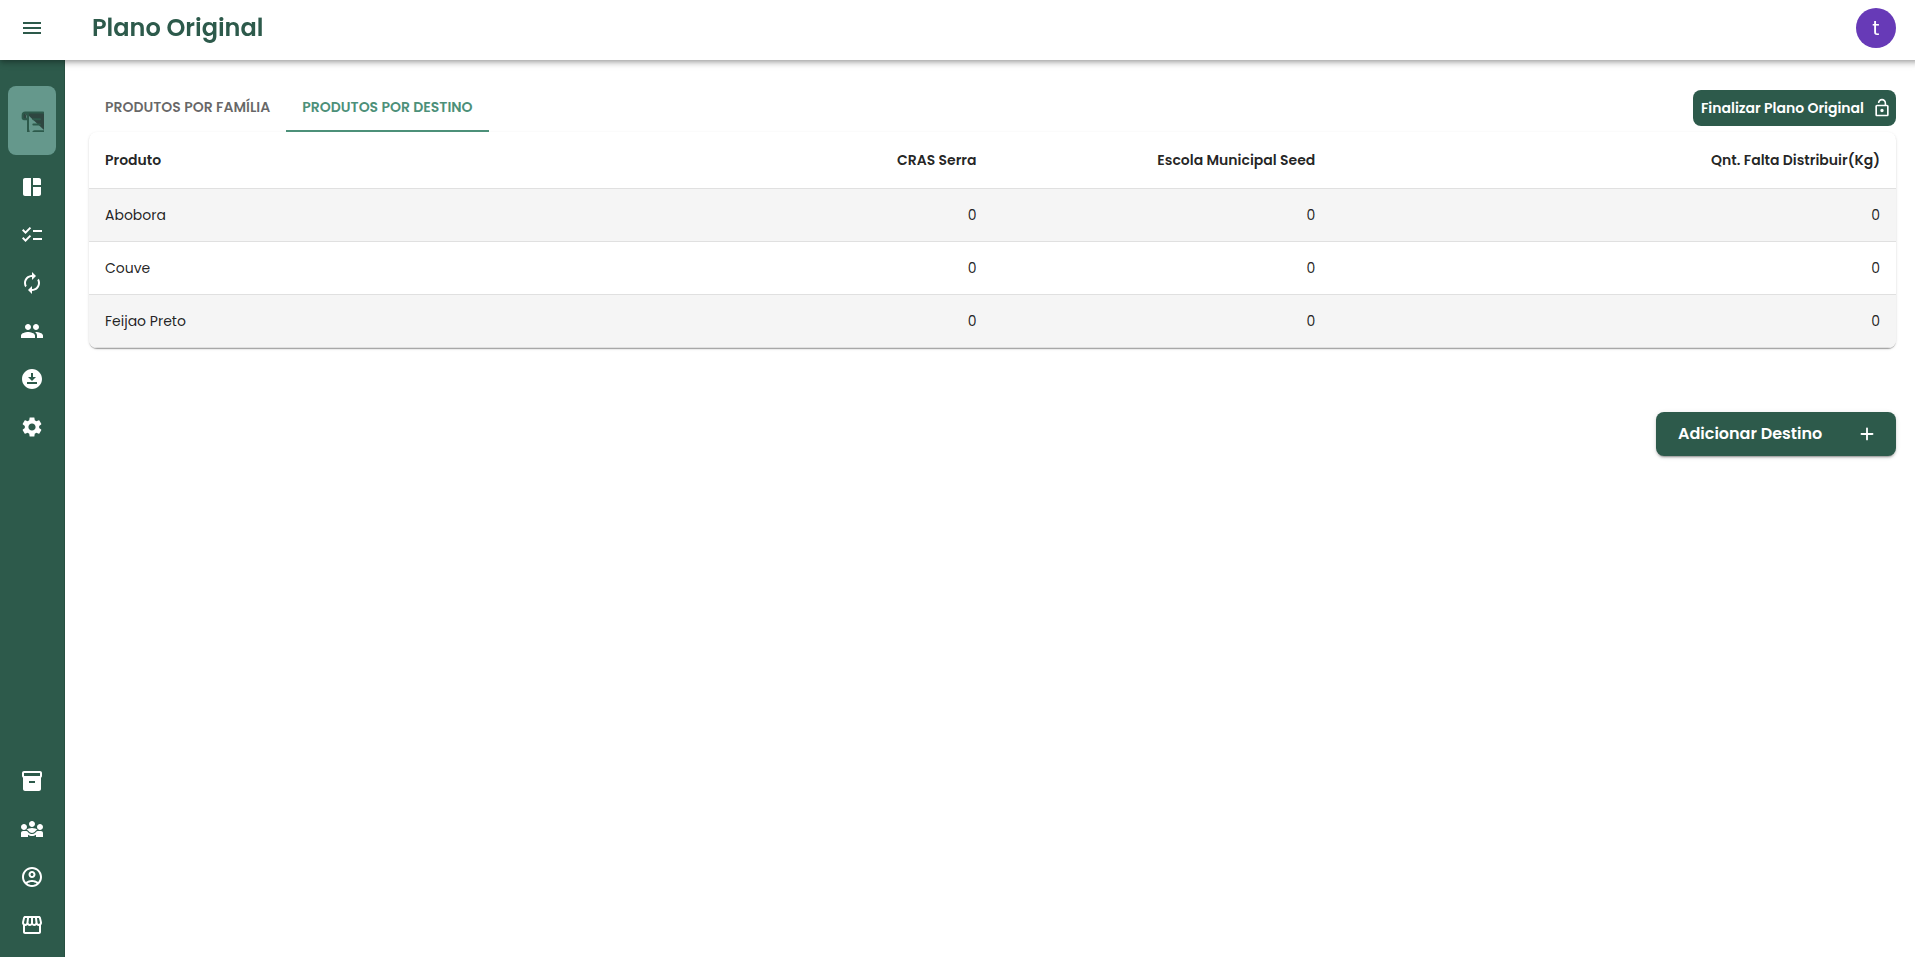
\includegraphics[width=1\textwidth]{Imagens/chap05/destino-semi-preenchido.png}
    \caption{Plano original aba produto por destino parcialmente preenchido}
    \label{fig:plano-original-destino}
\end{figure}

 \begin{figure}[H]
    \centering
    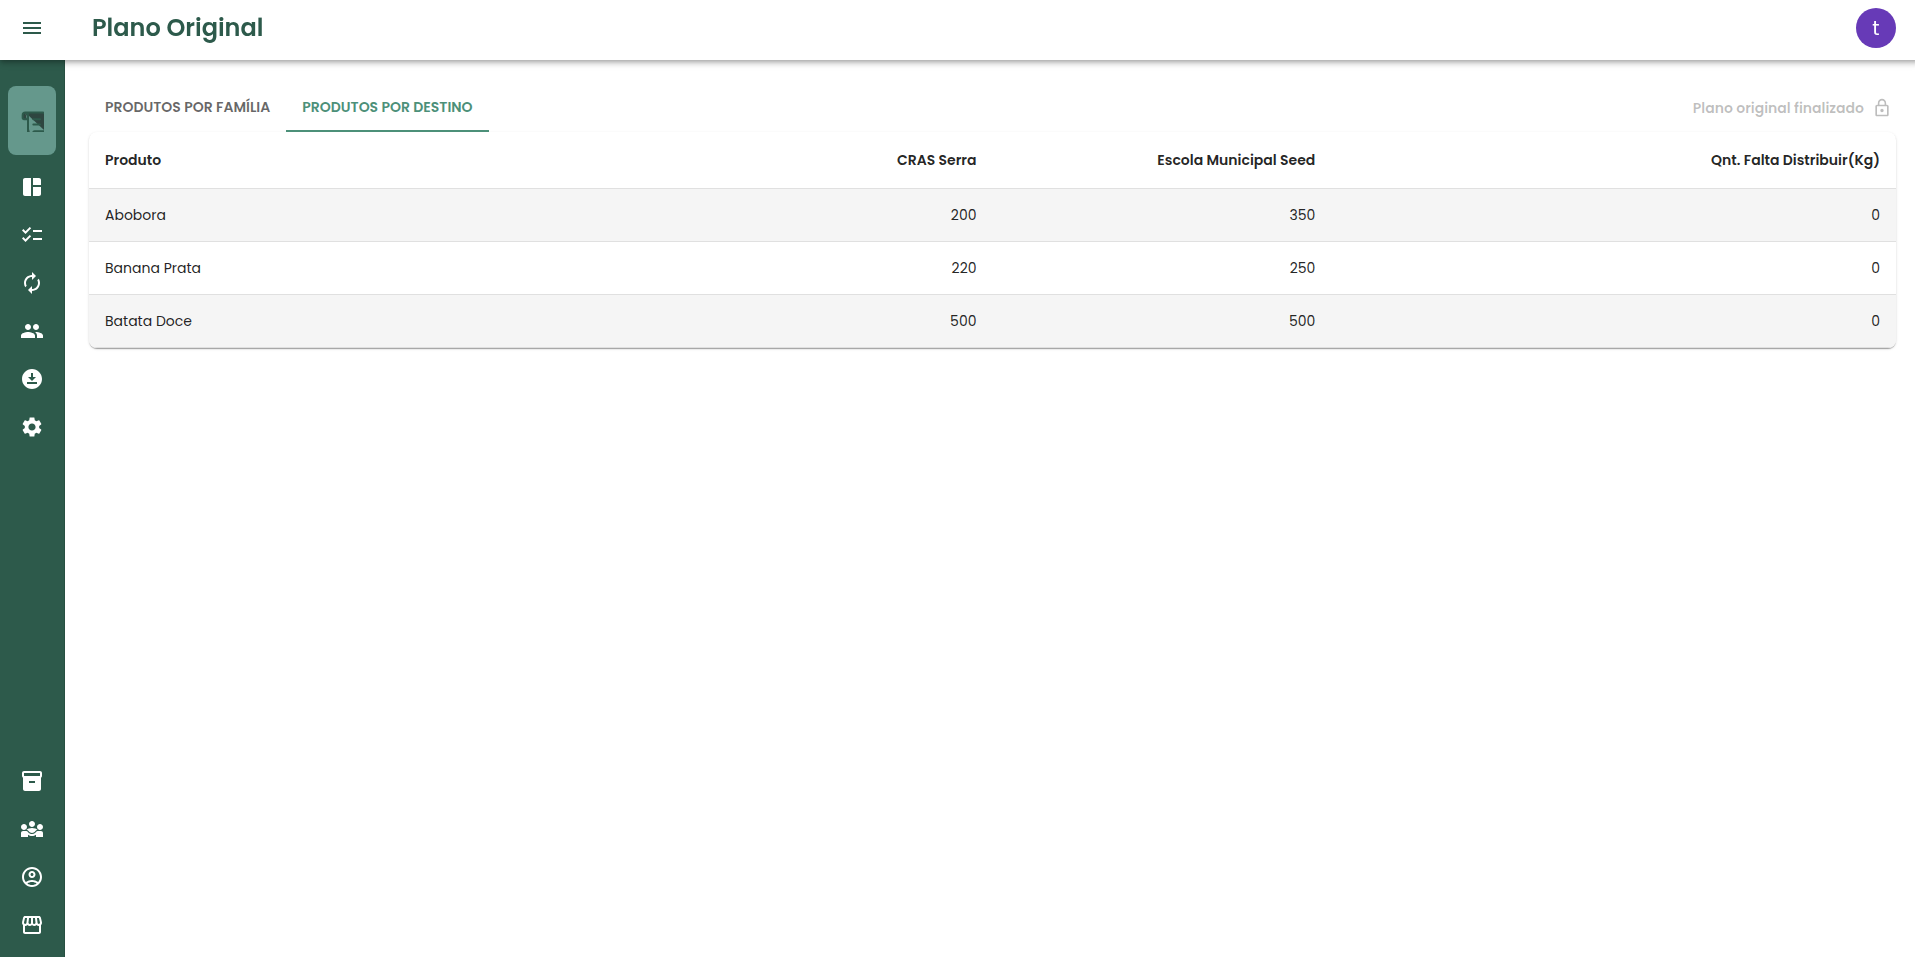
\includegraphics[width=1\textwidth]{Imagens/chap05/destino_plano_orignal.png}
    \caption{Plano original aba produto por destino completo}
    \label{fig:plano-original-destino-completo}
\end{figure}

Após a finalização do plano original, inicia-se a etapa de acompanhamento do andamento do edital por meio da tela de ciclos de entrega. Nessa tela, o coordenador pode criar os ciclos, definindo suas datas de início e fim, além de registrar a quantidade de produtos entregue por cada família e a quantidade destinada a cada local de entrega.

A Figura~\ref{fig:ciclo-entrega} exemplifica os três status possíveis dos ciclos já criados. Nessa tela, observa-se também a existência de dois controles principais: um relacionado às famílias e outro aos destinos. No controle de famílias, o coordenador registra as entregas realizadas em cada ciclo, informando a quantidade de produtos entregue por cada família. Para auxiliar esse processo, a tabela apresenta uma coluna de apoio que indica a quantidade ainda faltante de cada produto, considerando os valores definidos previamente no plano original.

O controle de destinos possui funcionamento semelhante. Nele, o coordenador define a quantidade de produtos que será encaminhada para cada destino em determinado ciclo. Ao lado das informações de entrega, o sistema apresenta a quantidade total prevista para cada destino ao longo do edital, permitindo acompanhar se a distribuição está de acordo com o plano original. Além disso, ao lado do nome de cada destino, há um botão para baixar o relatório necessário à comprovação da entrega daquele ciclo.

Assim como ocorre na página do plano original, o ciclo de entrega pode ser finalizado antes da data prevista para o seu encerramento. Ao finalizar um ciclo, seu status é alterado e a edição das informações passa a ser bloqueada, garantindo maior controle sobre os dados registrados. No entanto, diferentemente do plano original, um ciclo finalizado pode ser reaberto, caso seja necessário corrigir ou complementar alguma informação posteriormente.


\begin{figure}[H]
    \centering
    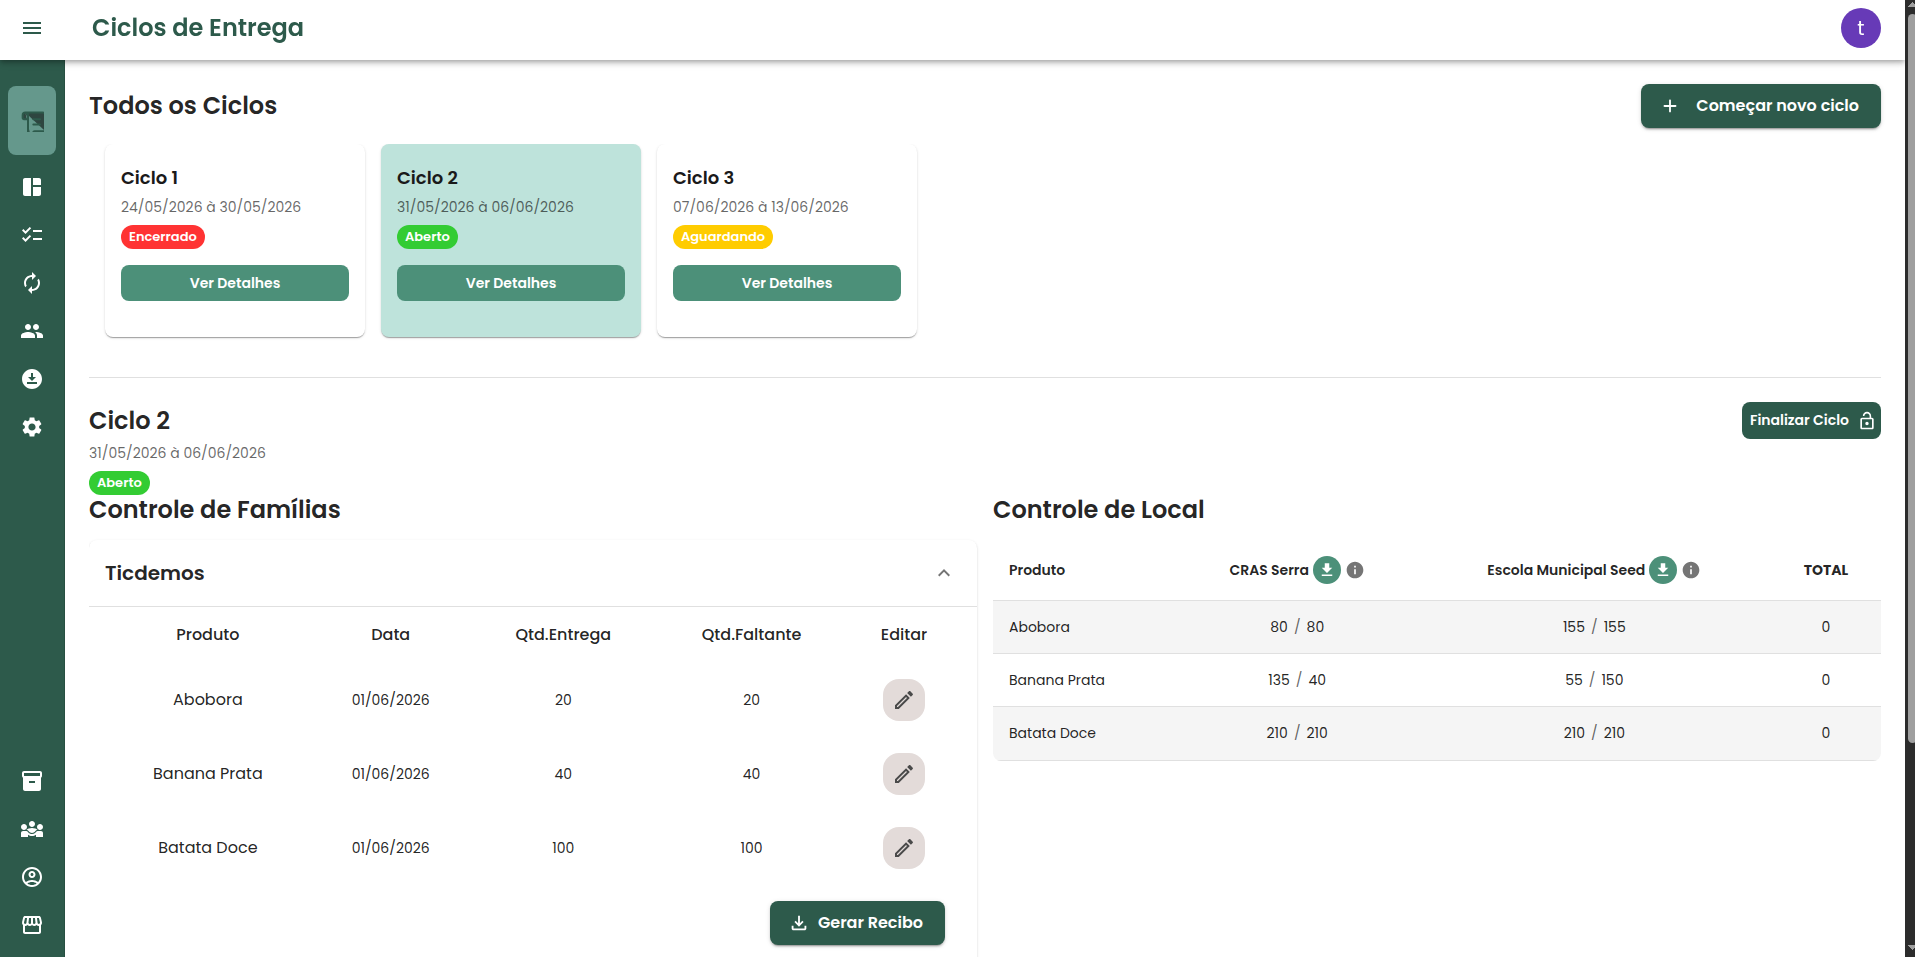
\includegraphics[width=1\textwidth]{Imagens/chap05/tela_ciclos_entrega.png}
    \caption{Ciclos e Entregas}
    \label{fig:ciclo-entrega}
\end{figure}


Após a finalização do ciclo de entrega, o coordenador pode baixar os relatórios referentes àquele período para cada destino. A Figura~\ref{fig:relatorios} apresenta, por meio de cards, todos os destinos vinculados ao edital, juntamente com suas principais informações. Em cada card, é possível baixar o relatório de recebimento de alimentos, utilizado para comprovar as entregas realizadas naquele destino. Dessa forma, os documentos são gerados pelo coordenador, mas registram informações que servem como comprovação das entregas feitas pelas famílias agricultoras.

Além disso, nessa mesma tela, há o botão para baixar o relatório de pagamento. Esse relatório sintetiza as entregas realizadas por família, apresentando a quantidade entregue e o valor que cada uma deverá receber ao final do ciclo.


\begin{figure}[H]
    \centering
    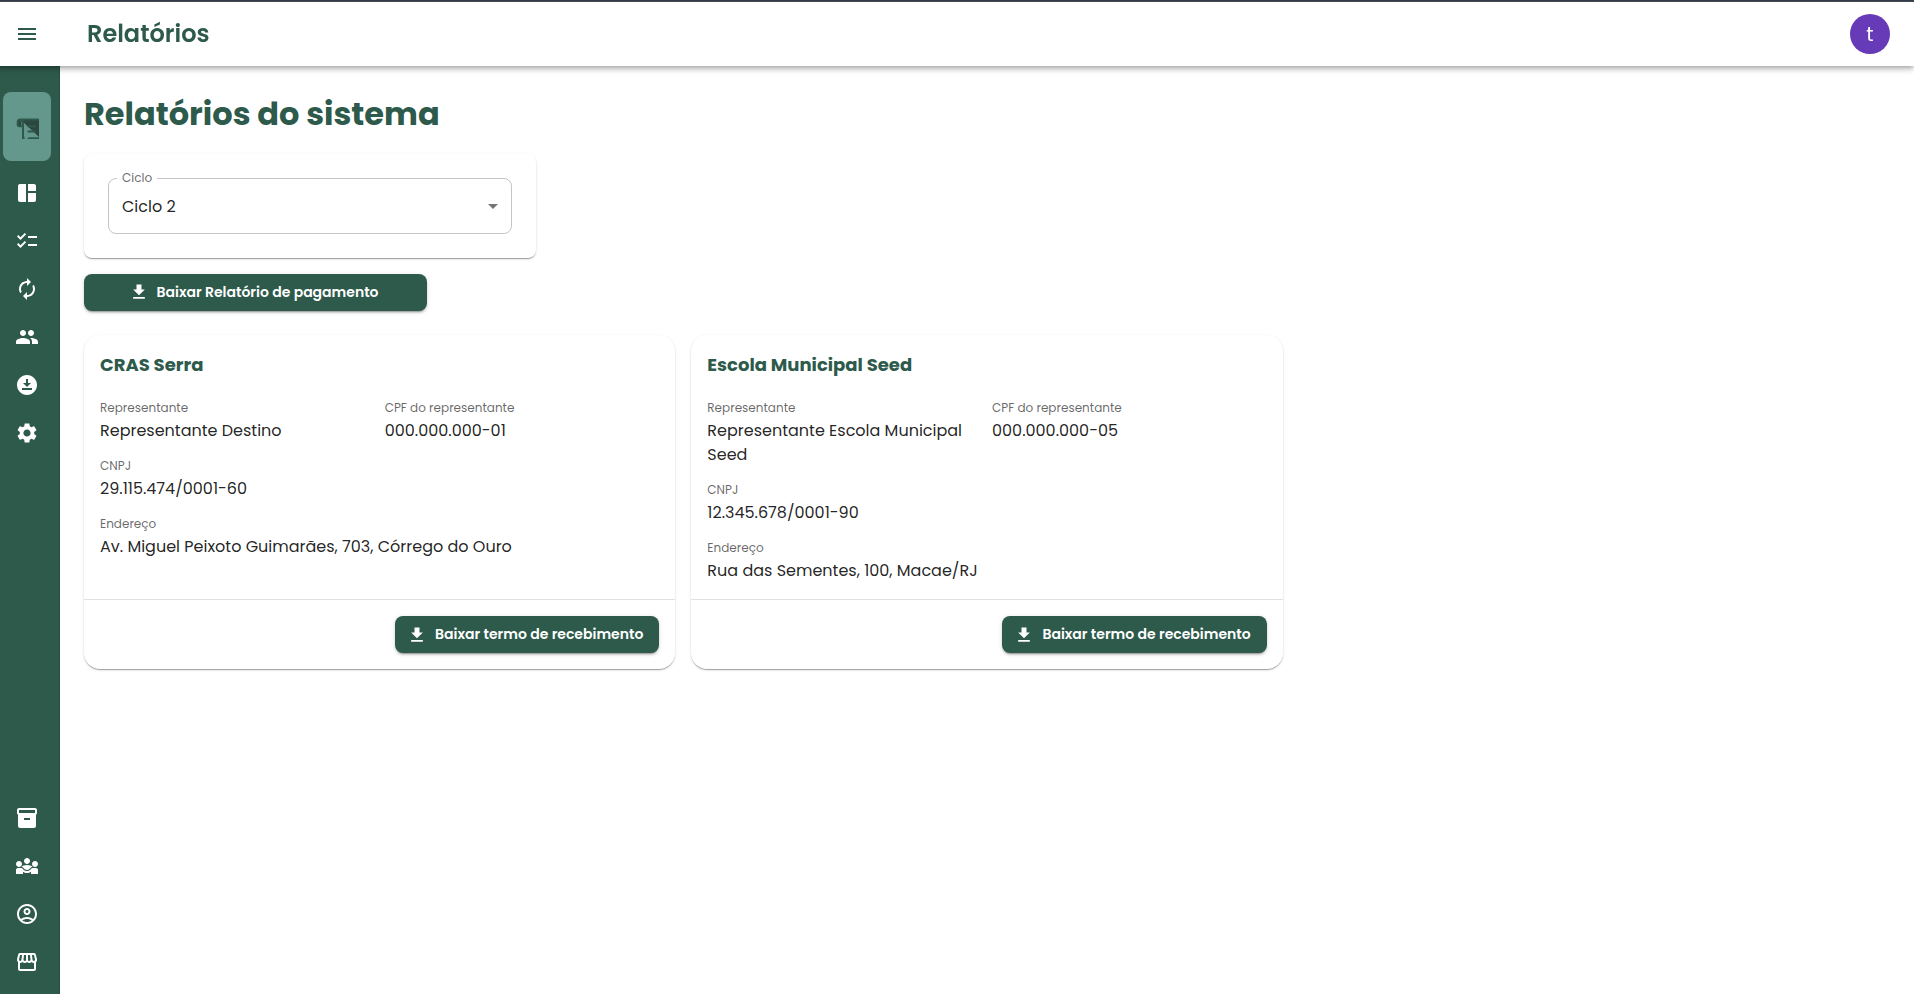
\includegraphics[width=1\textwidth]{Imagens/chap05/tela_relatorios.png}
    \caption{Relatórios}
    \label{fig:relatorios}
\end{figure}

Com o objetivo de permitir o acompanhamento individual de cada família, o coordenador tem acesso à tela de detalhes da família. Nessa tela, os dados dos ciclos de entrega são organizados por família, permitindo visualizar quanto foi entregue em cada ciclo e o valor total recebido. Além disso, o sistema possibilita a geração do recibo referente àquele ciclo para a família selecionada.

Na última coluna da tabela, há um recurso de apoio ao coordenador, que apresenta o acompanhamento acumulado das entregas ao longo dos ciclos. Essa coluna indica a quantidade de alimentos já entregue pela família e a quantidade ainda faltante em relação ao que foi definido no plano original. Na última célula da tabela, são apresentados o valor já recebido pela família e o valor que ainda deverá ser recebido até o final do edital. Abaixo, na Figura~\ref{fig:detalhes-familia} segue um exemplo.

\begin{figure}[H]
    \centering
    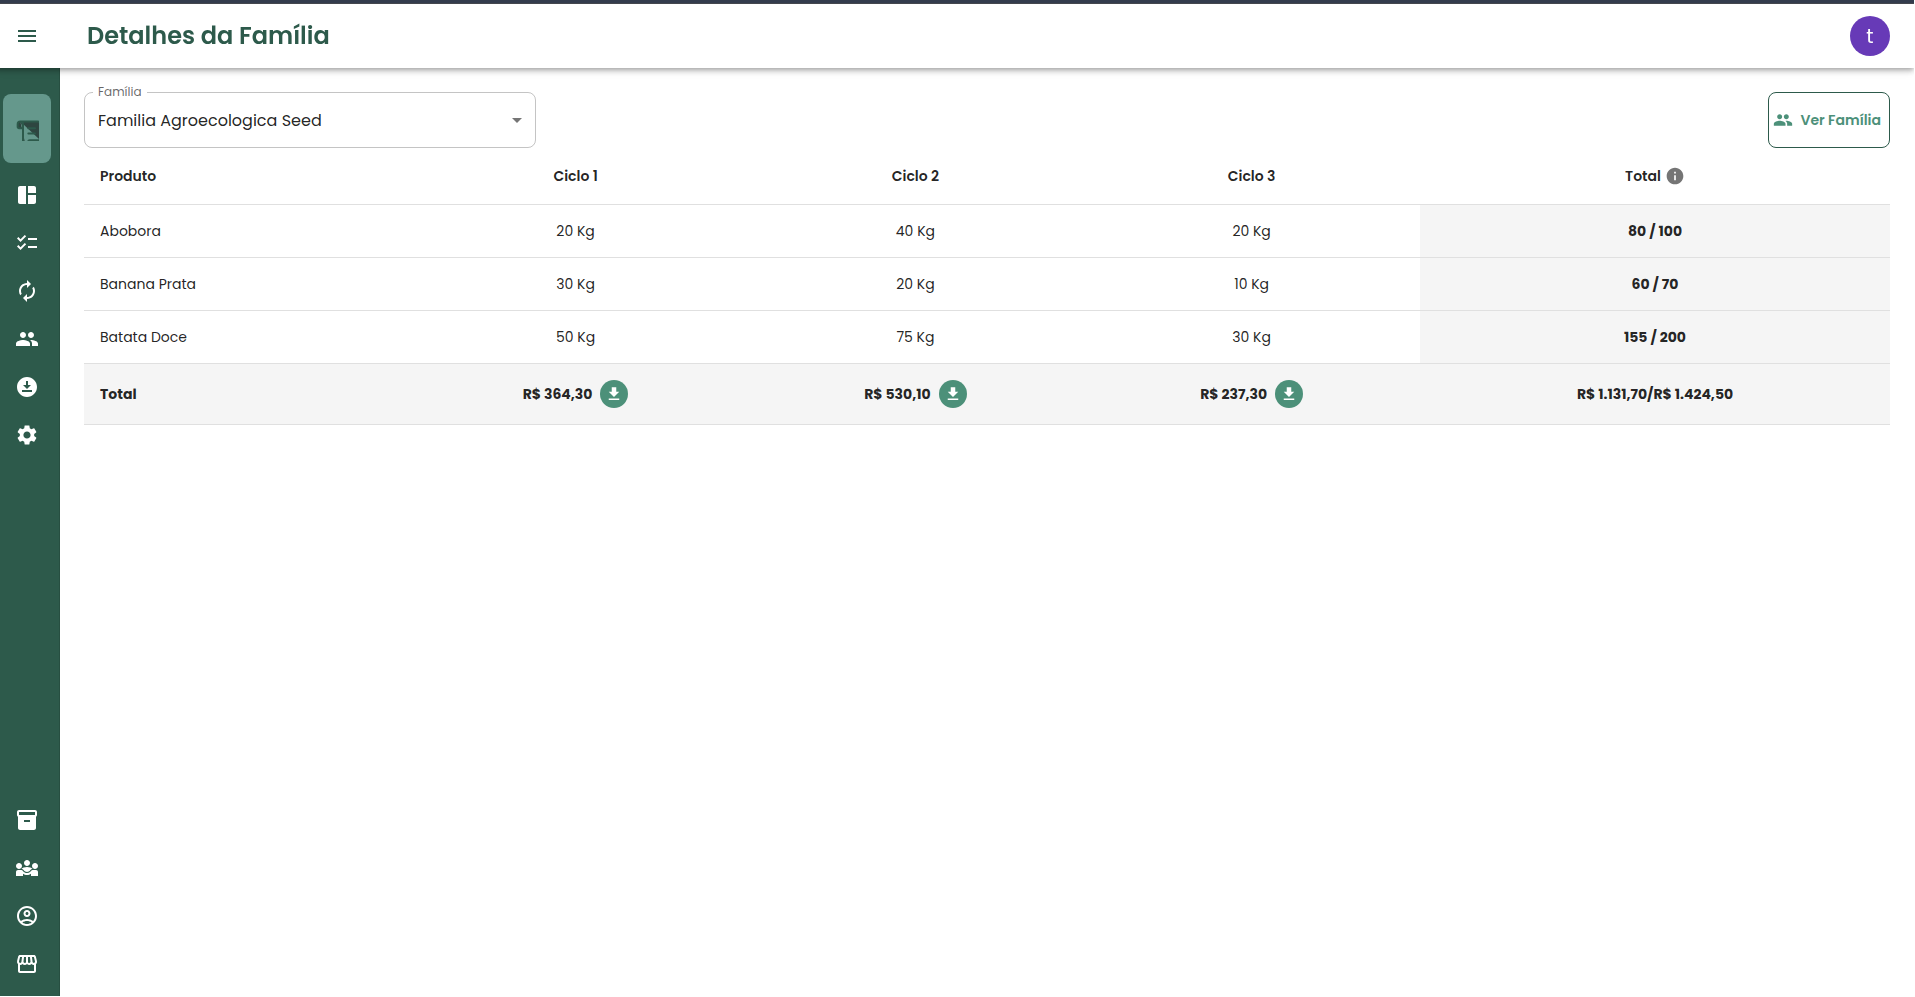
\includegraphics[width=1\textwidth]{Imagens/chap05/tela_detalhes_familia.png}
    \caption{Detalhes da família}
    \label{fig:detalhes-familia}
\end{figure}

Para verificar informações gerais do edital, o sistema possui a tela de configuração, onde há um resumo do cadastro inicial, com informações de início e fim, assim como a quantidade limite de quilos de alimento por entrega e por fim, um card que ao ser clicado redireciona para o plano original. Abaixo segue a imagem com exemplo.

\begin{figure}[H]
    \centering
    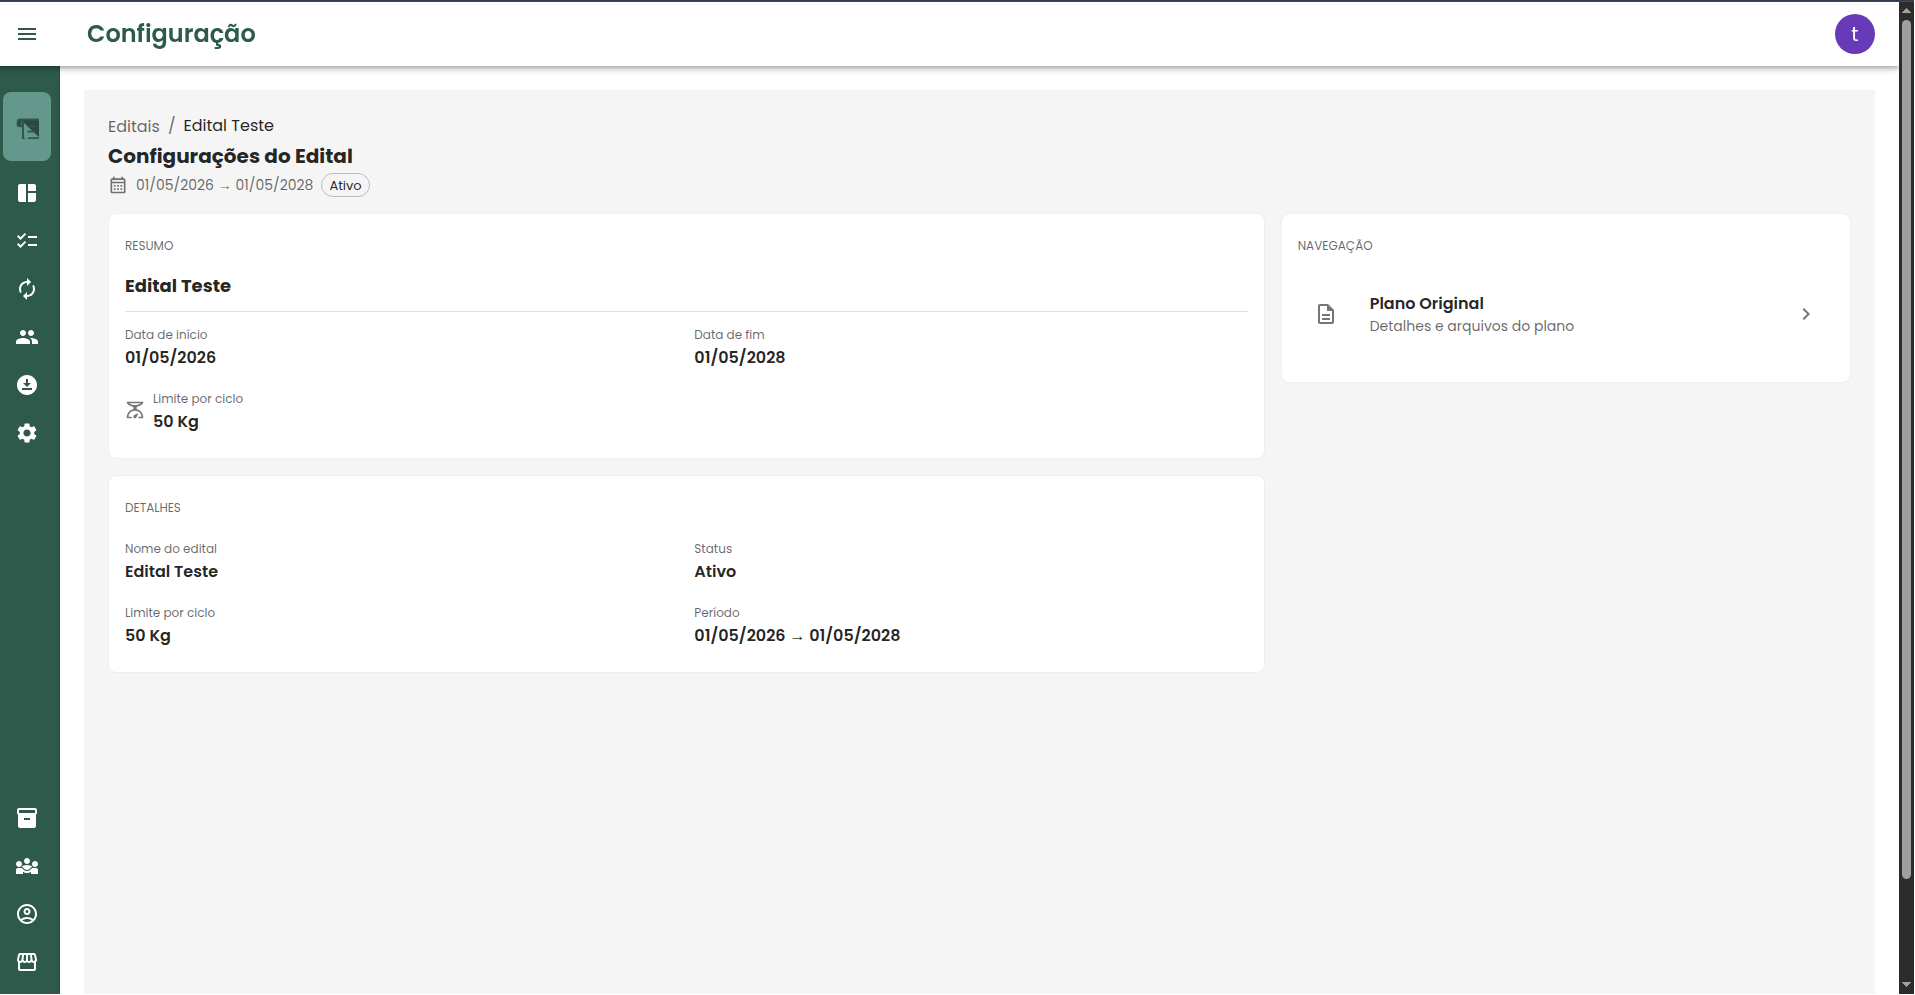
\includegraphics[width=1\textwidth]{Imagens/chap05/tela_configuracao_edital.png}
    \caption{Configuração}
    \label{fig:configuracao}
\end{figure}

Após a finalização do plano original, o dashboard passa a ser preenchido automaticamente com as informações necessárias para acompanhar o andamento do edital. A Figura~\ref{fig:dashboard} apresenta um exemplo da visualização dessa tela.

O dashboard é composto por indicadores que sintetizam o progresso. Entre essas informações, são apresentados os produtos cadastrados, a quantidade já entregue e a quantidade prevista no plano original. Ao interagir com um produto, por meio de um clique, o coordenador consegue visualizar a porcentagem de entrega correspondente a cada família, permitindo um acompanhamento mais detalhado da execução do edital.

Nessa mesma tela, também são apresentados dois gráficos relacionados ao andamento dos ciclos de entrega. O primeiro gráfico detalha quais produtos foram entregues em cada ciclo e suas respectivas quantidades. O segundo gráfico, localizado mais à direita, apresenta a quantidade total de alimentos entregue por ciclo, permitindo uma visão geral da evolução das entregas ao longo do edital.

\begin{figure}[H]
    \centering
    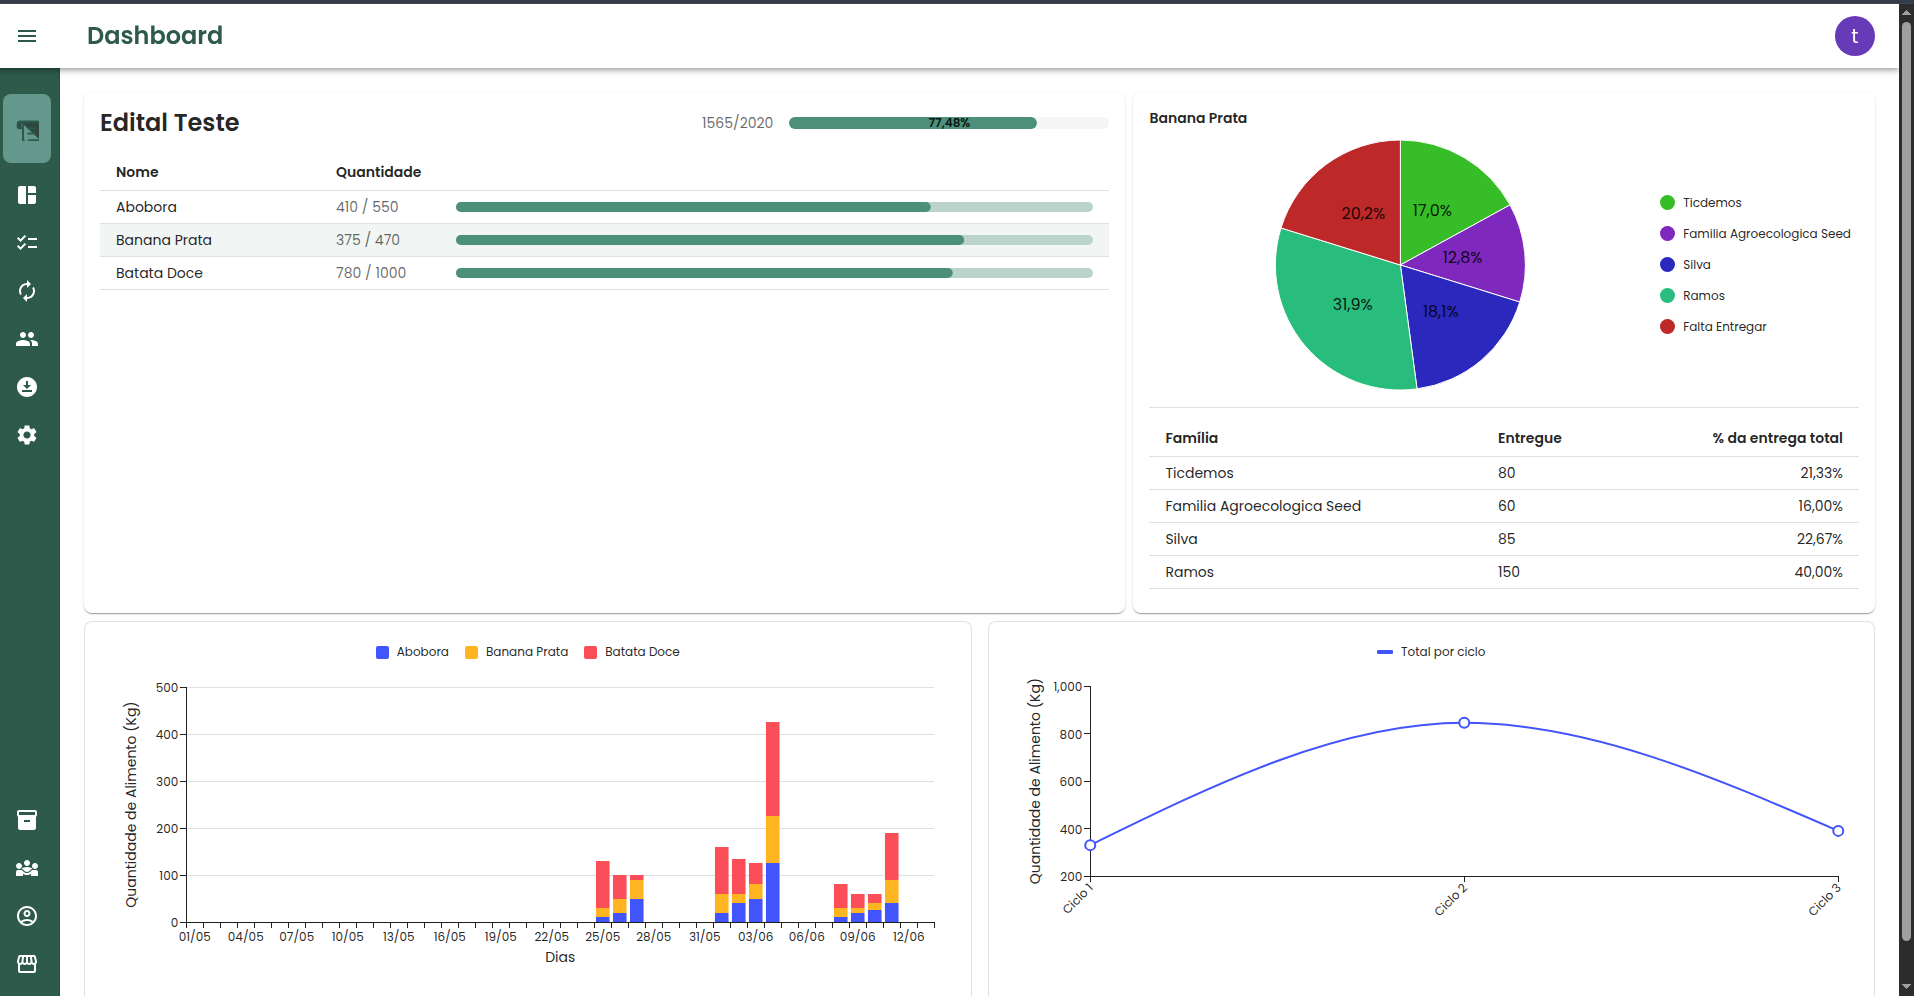
\includegraphics[width=1\textwidth]{Imagens/chap05/dashboard.png}
    \caption{Dashboard}
    \label{fig:dashboard}
\end{figure}

Com o objetivo de atender a informações comuns a diferentes editais, o sistema possui entidades globais, representadas nas figuras a seguir. Essas entidades evitam a repetição desnecessária de dados.

Na Figura~\ref{fig:produtos-globais}, são apresentados os produtos globais cadastrados no sistema. Cada edital pode possuir sua própria representação desses produtos, o que permite utilizar uma mesma informação base, mas com valores e quantidades específicas para cada edital. Dessa forma, um mesmo produto pode estar presente em diferentes editais, porém com preço, quantidade prevista e demais configurações próprias de cada chamada.

Além dos produtos, o sistema também possui como entidades globais os coletivos e os destinos, representados, respectivamente, pelas figuras~\ref{fig:coletivos-globais} e~\ref{fig:destinos-globais}. Esses cadastros permitem organizar informações utilizadas em diferentes partes do sistema, facilitando o gerenciamento e a vinculação dessas entidades aos editais.

Por fim, há também o cadastro de usuários, representado na Figura~\ref{fig:usuario-globais}. A partir dos usuários cadastrados, o sistema permite organizar os participantes e associá-los às famílias correspondentes, respeitando sua vinculação ao coletivo e à chamada pública correspondente.


\begin{figure}[H]
    \centering
    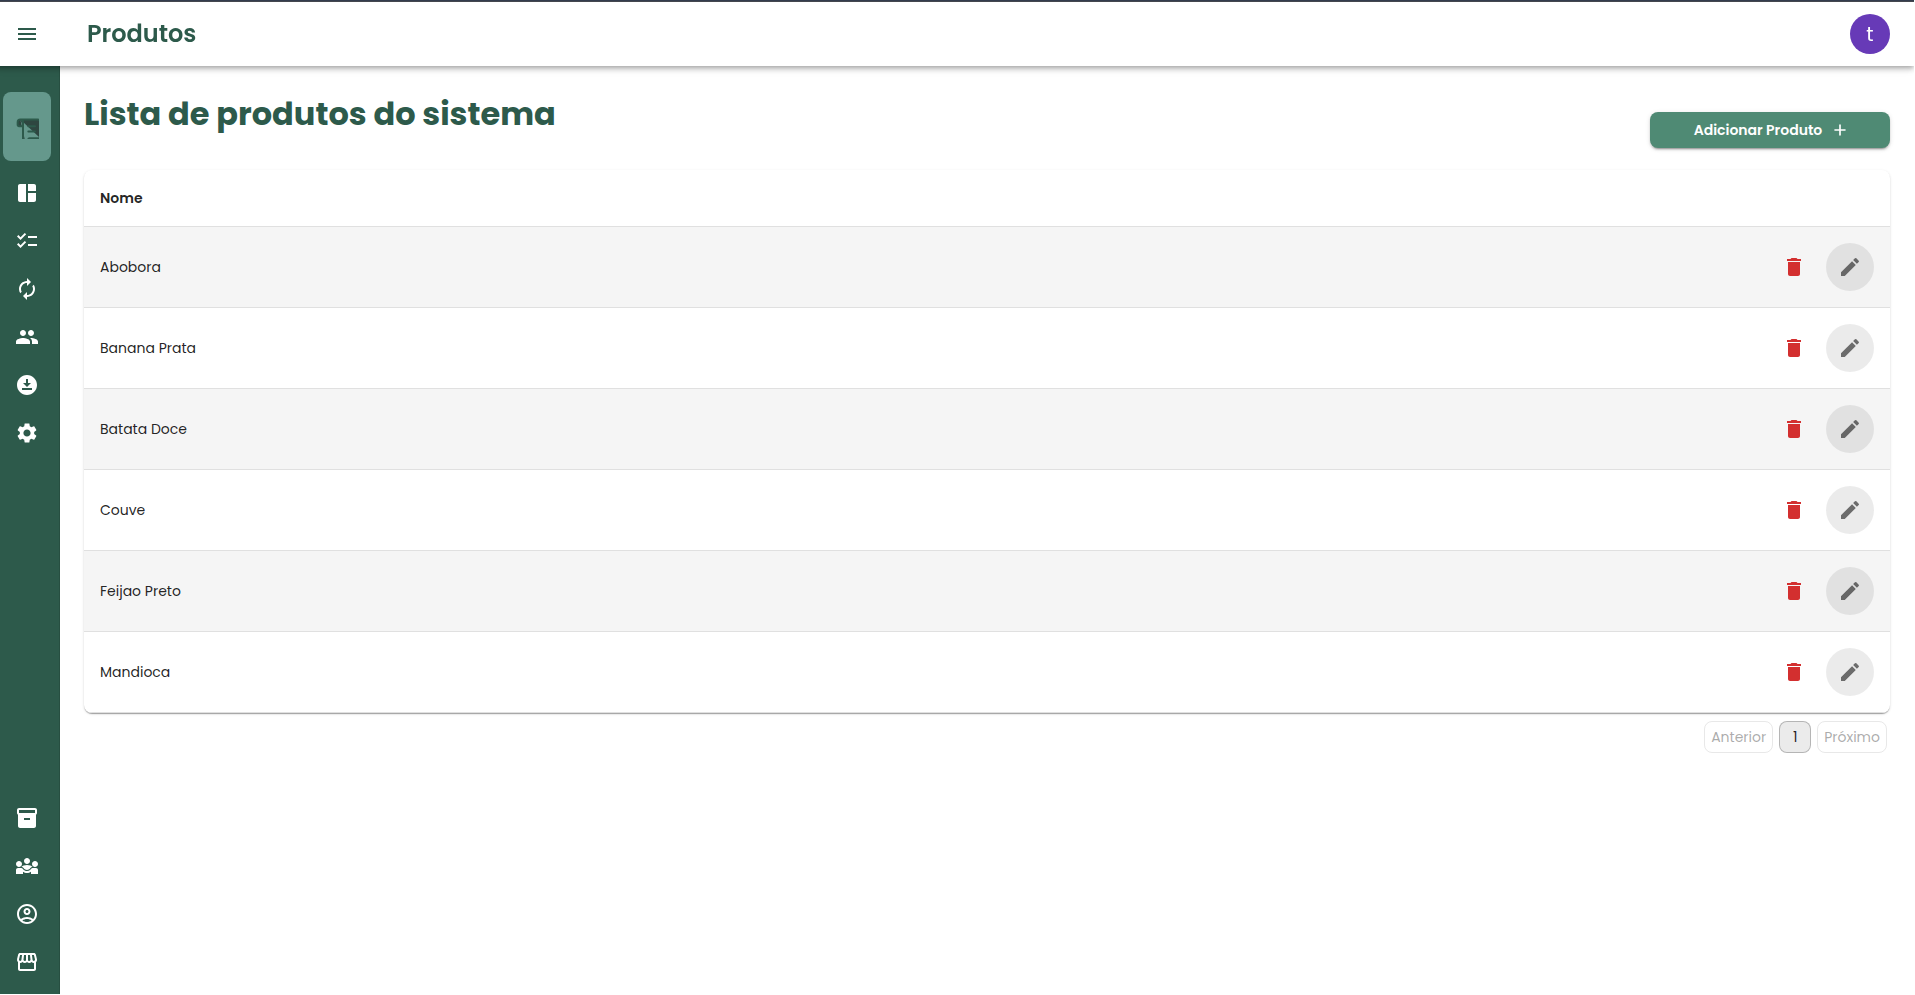
\includegraphics[width=1\textwidth]{Imagens/chap05/produtos_globais.png}
    \caption{Produtos}
    \label{fig:produtos-globais}
\end{figure}

\begin{figure}[H]
    \centering
    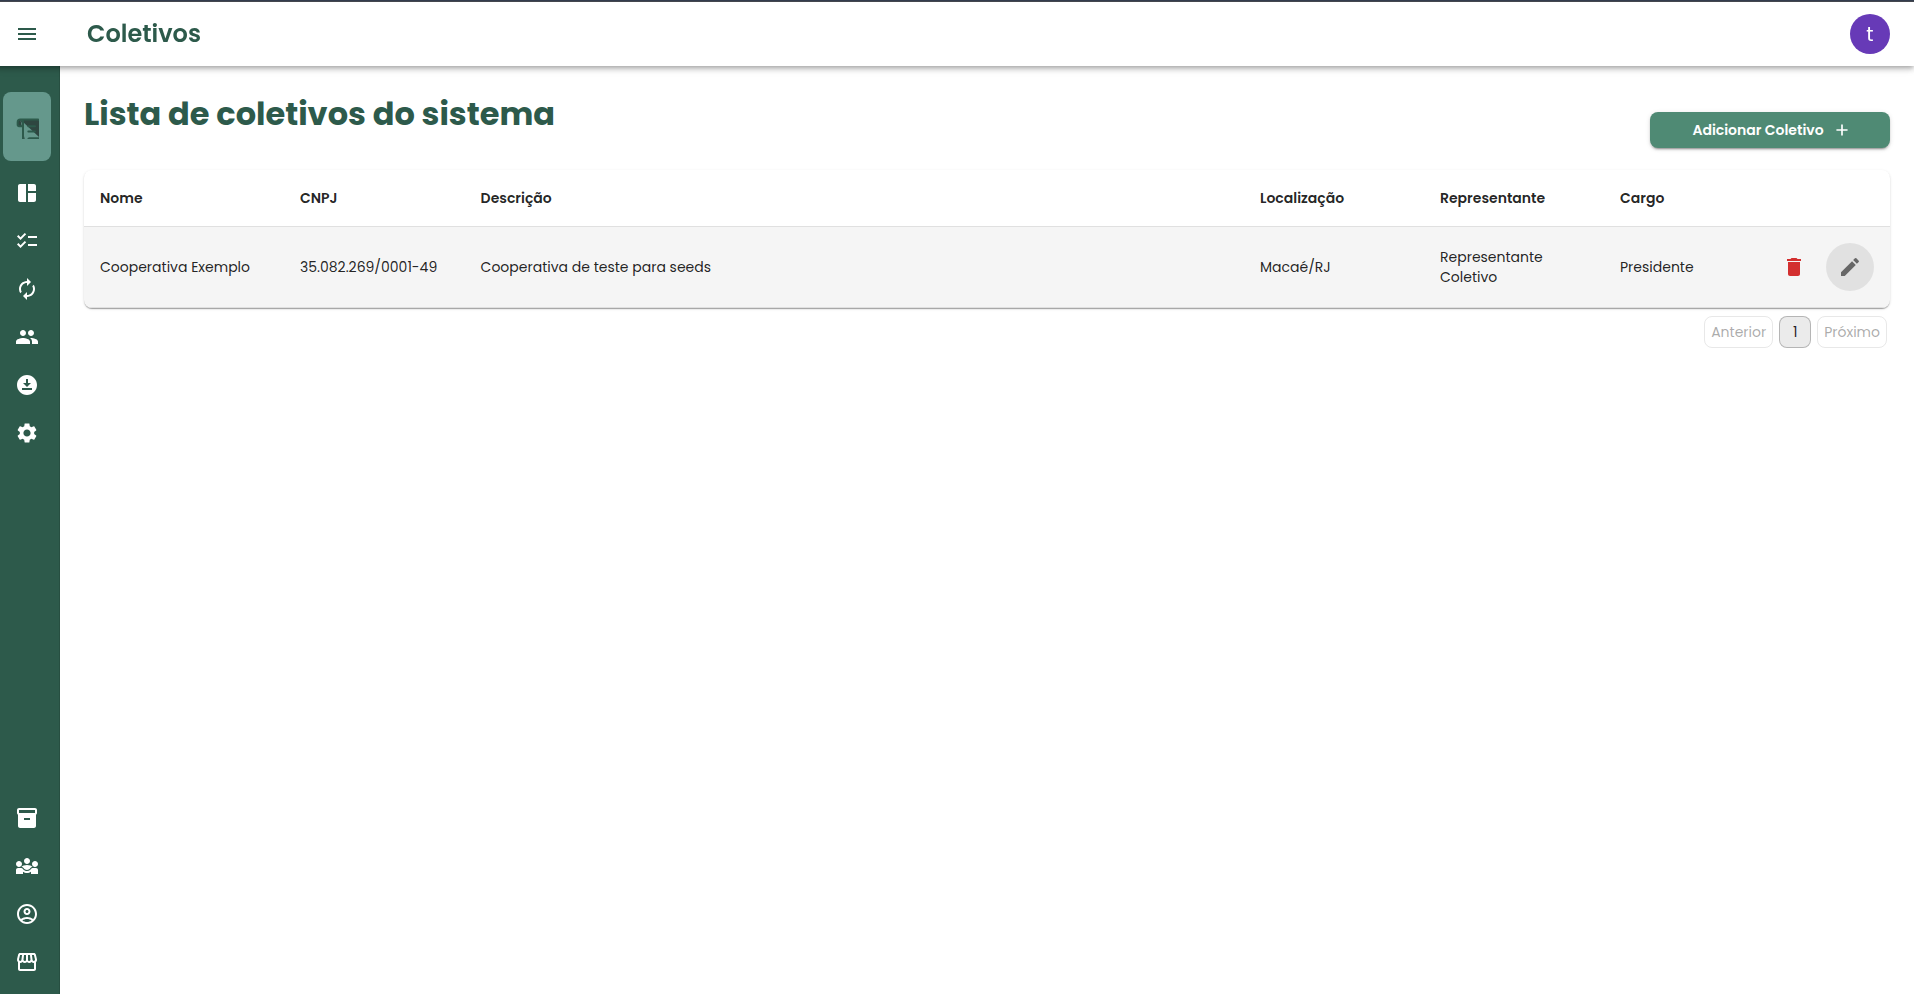
\includegraphics[width=1\textwidth]{Imagens/chap05/tela_coletivos.png}
    \caption{Coletivos}
    \label{fig:coletivos-globais}
\end{figure}

\begin{figure}[H]
    \centering
    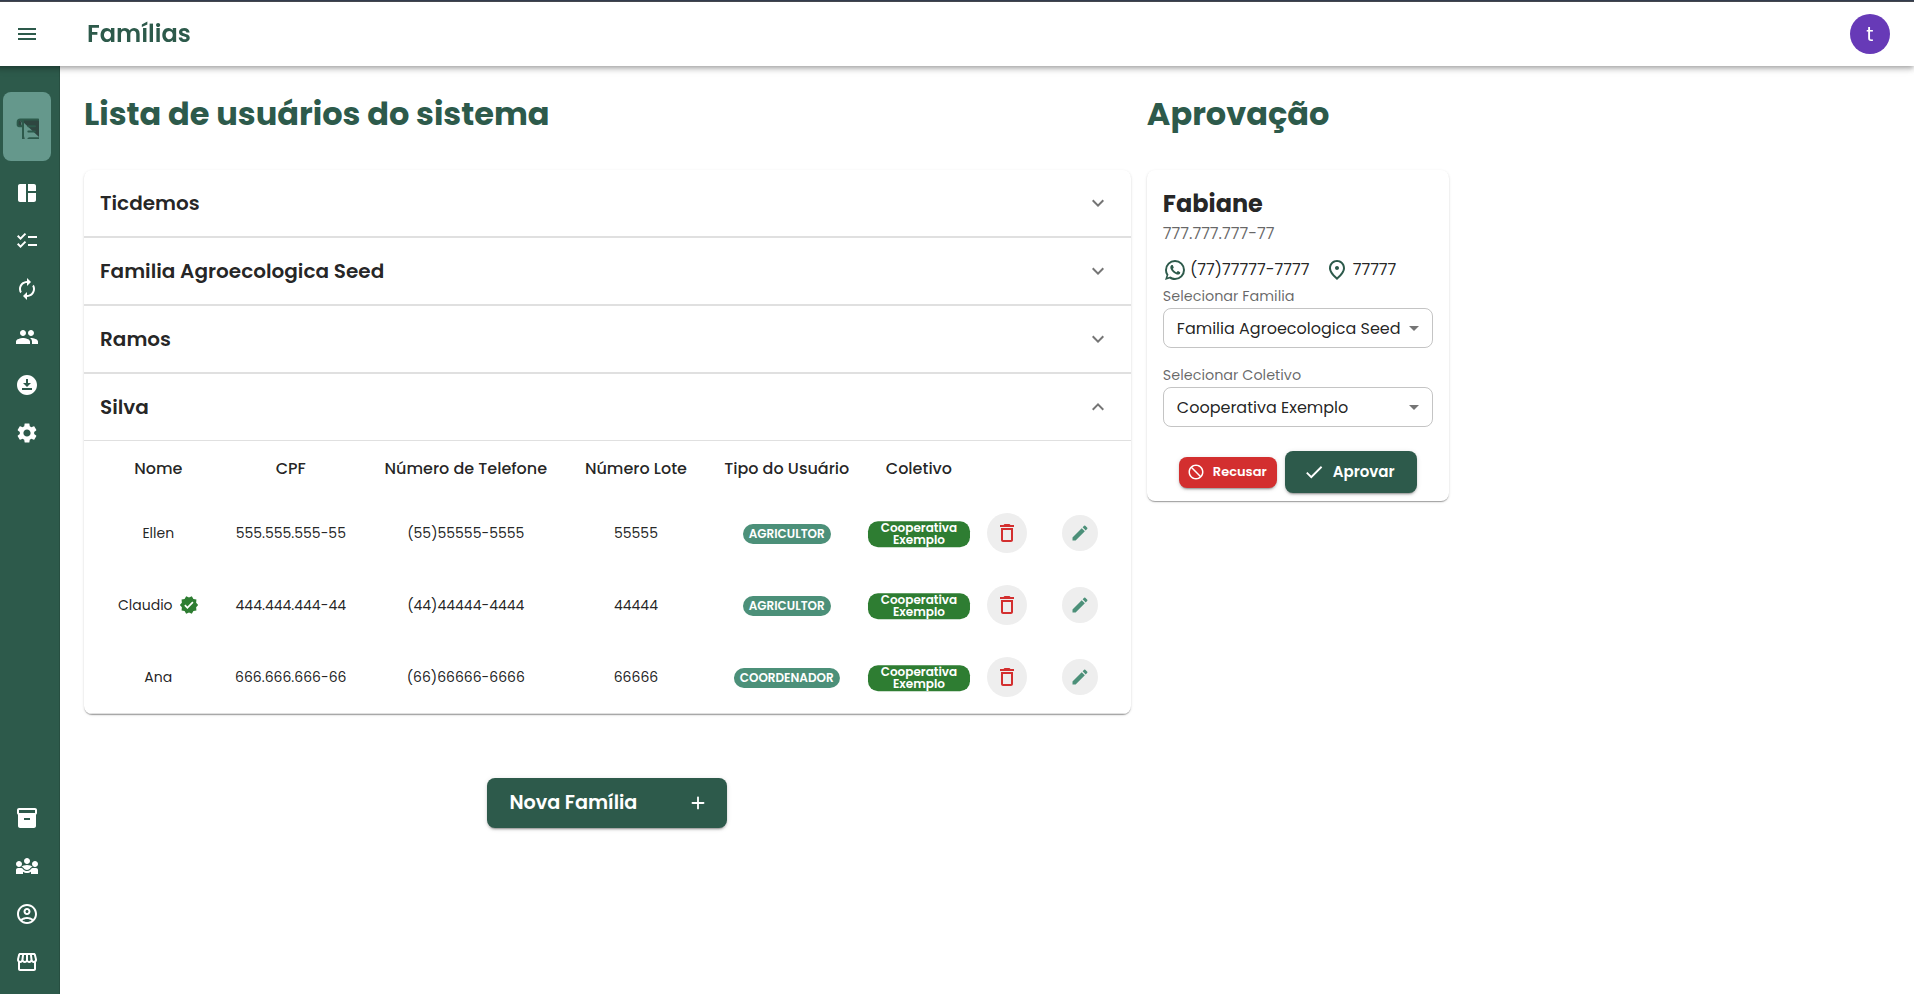
\includegraphics[width=1\textwidth]{Imagens/chap05/tela_usuarios_sistema.png}
    \caption{Usuários}
    \label{fig:usuario-globais}
\end{figure}

\begin{figure}[H]
    \centering
    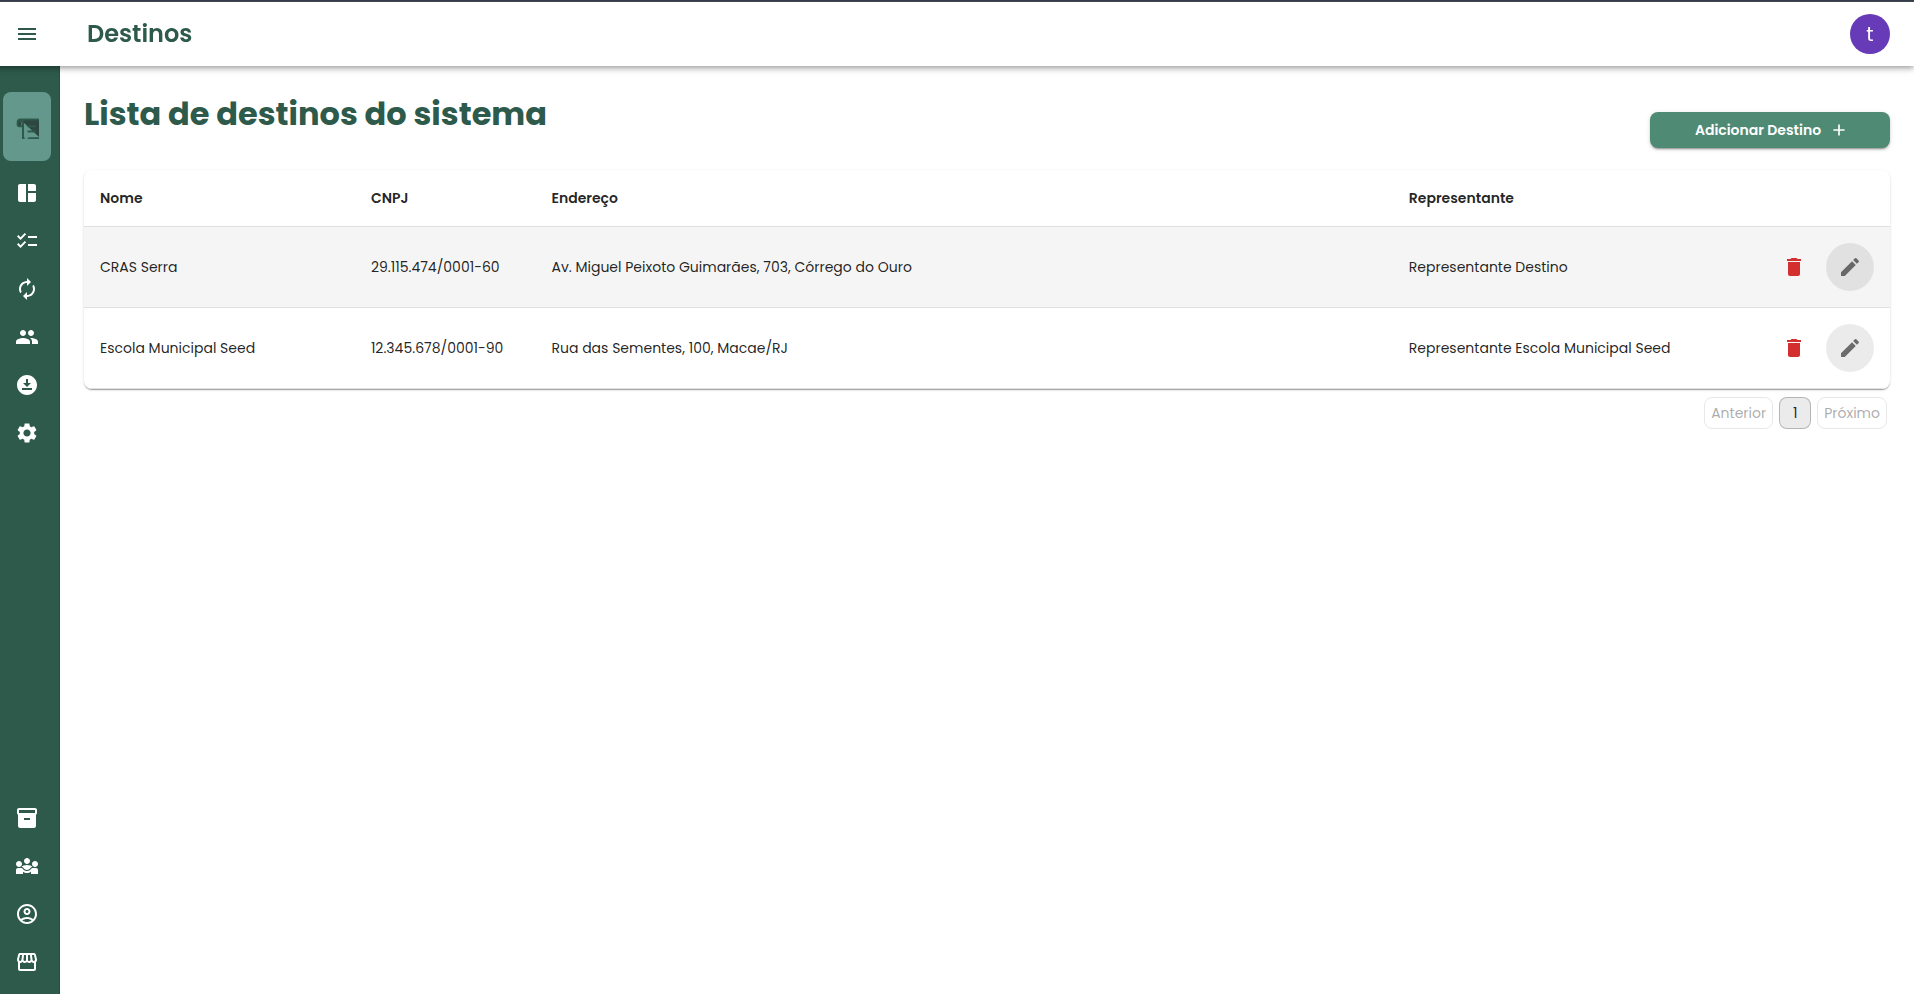
\includegraphics[width=1\textwidth]{Imagens/chap05/tela_destino_sistema.png}
    \caption{Destinos}
    \label{fig:destinos-globais}
\end{figure}

\section{Integração e Deploy}

Durante o desenvolvimento do sistema, foi utilizado o Git como ferramenta de controle de versão, permitindo o acompanhamento das alterações realizadas no código-fonte e facilitando o trabalho colaborativo entre os desenvolvedores. Para o armazenamento remoto dos repositórios, foi utilizado o GitLab, que também oferece recursos de integração contínua e entrega contínua.

Com o objetivo de apoiar a integração contínua de novas funcionalidades e padronizar o processo de construção da aplicação, foi configurado, em cada projeto, um arquivo chamado \texttt{.gitlab-ci.yml}. Esse arquivo é responsável por definir as etapas executadas automaticamente pelo GitLab CI/CD, como a verificação do código, acionamento de testes automatizados, a execução do build e a geração de uma nova imagem Docker. No backend, esse processo utiliza o Maven para executar as etapas de teste e construção da aplicação. No frontend, o processo utiliza o Vite para gerar a versão de produção da interface. Neste primeiro momento a aplicação possui somente testes automatizados para pontos essenciais e comportamentos críticos do sistema. Após a criação da imagem, ela é publicada no Docker Hub, possibilitando que a versão mais recente da aplicação esteja disponível para implantação no ambiente de homologação.

O ambiente de homologação da aplicação encontra-se em uma VPS hospedada na Hostinger. Nesse ambiente, o deploy ainda é realizado de forma manual. Para isso, existe um script no servidor responsável por remover as imagens locais dos containers, baixar as versões mais recentes publicadas no Docker Hub e executar novamente o Docker Compose, fazendo com que os serviços da aplicação sejam atualizados e disponibilizados online.



